\section{Introduction}

To understand the context and strategies of modern Russian computational propaganda, it is useful to first take a look to the past, many of the same dynamics are still in effect.
Russia is and was a country of many peoples with both Western and Eastern influences dominated by a small authoritarian elite.
This environment was the breeding ground for early modern revolutionary groups and propaganda.
Narodnaya Volya (People's Will) was founded in 1879 and heavily influenced by ``propaganda of the deed'' which advocated for, among other actions, terrorist attacks \cite[p. 5]{hoffman2017}.
Though an ``essentially contested concept'', the defining characteristic of terrorism contra other forms of political violence is (according to most definitions) the centrality of propaganda \cite[p. 86]{schmid2011}.
This became an especially useful strategy with the rise of modern mass media and a literate middle class which could rapidly disseminate news, ideas, and fear.

Narodnaya Volya is probably best known for the assassination of Tsar Alexander II in 1881.
Vladimir Lenin's older brother Alexander Ulyanov was executed after a failed plot on the life of the next tsar by a later iteration of the group.
His death is often cited as a radicalizing influence on Lenin \cite[p. 60]{service2000}.
The early Bolsheviks matured and were brutalized in this environment dominated by terrorism, conspiracy, and propaganda; they used these tools upon acquiring power.
The newspaper Pravda (``Truth'') was recreated in 1917 with Kamenev, Stalin, and Bukharin as editors during and after the revolution and remained an official publication of the Soviet regime until the collapse of the USSR \cite[p. 209]{trotsky2008} \cite[p. 43]{cohen1980}.
Lenin is known for The Red Terror, an explicit policy of marginalization, dehumanization, and removal of groups such as wealthy peasants (kulaks), clergy, intellectuals, and political opponents.
The Cheka (secret police) was established to meet counterrevolutionary threats, Soviet press encouraged the violence, and Old Bolsheviks like Trotsky and Zinoviev defended it as necessary \cite{melgunoff1927, trotsky2017} \cite[p. 114]{leggett1981}.
Similar programs existed well into Stalin's reign; Kamenev, Bukharin, and Zinoviev became victims of The Great Terror of the 1930s; Trotsky was assassinated in Mexico City in 1941.

Under the head of the Cheka, Felix Dzerzhinsky, a department for disinformation (dezinformatsiya) was established in 1923 \cite[p. 18]{rid2020}.
The term agitprop similarly came into use after the establishment of a department for agitation and propaganda; these departments small parts of a propaganda ``machine'' \cite{kenez1985}.
Soviet propaganda made use of common techniques such as cults of personality, indoctrination of youth, politicized cinema and art, and class and ethnic hatred.
However, the Soviet use of disinformation and ``active measures'' was unmatched in scale and sophistication.
During the Cold War American hypocrisy over Jim Crow laws, lynchings, and Vietnam were harnessed; as late as the 1980s Soviet media was spreading the conspiracy theory that AIDS was intentionally engineered by the US government \cite[ch. 11, 22]{rid2020}.

The fall of the Soviet Union left a power vacuum which was filled by strongmen and oligarchs throughout the former republics.
As an officer in the KGB, Vladimir Putin was no stranger to the uses of information and disinformation and his transformation from a relative unknown to the president of Russia was greatly aided by the media campaigns of multiple oligarchs.
While many Soviet institutions ended, others survived through a facelift and rebranding.
The KGB, for example, remained largely intact as the SVR. 
Past propaganda tactics were appropriated including fakes and forgeries, reflexive control - turning the internal divisions of an opponent on itself, and active measures - clandestine operations to influence foreign governments, undermine domestic confidence, and degrade relationships with other countries.
The Rose Revolution in Georgia in 2003 and the Orange Revolution in Ukraine the following year convinced decision makers that Russia was losing soft power and influence over traditional buffer states in eastern Europe.
The establishment of Russia Today (now RT) in 2005 was part of an intentional campaign to recast the country as an underdog to the hegemony of the United States and the latter less as an enemy but rather as a competitor to be engaged by practical means \cite[pp. 21-24]{woolley2018}.
The US invasion of Iraq in 2003, war in Georgia in 2008, and the Arab Spring uprisings of 2011 were seen as further evidence of Western intervention requiring new strategies.

There is some truth to Western influence behind unrest in several of these states but a bigger factor, cited extensively, was the unexpected impact that new social media networks such as Twitter had as conduits of information, mobilization, and organization \cite{harlow2011, bruns2014}.
Russia was experiencing their reach, too.
By 2010, the vast majority of traditional media outlets in Russia such as TV, print, and radio were under government control.
During the 1990s a nascent tech industry grew due to the efforts of entrepreneurs taking advantage of market freedoms.
Whether due to Internet penetration being minuscule (as of 2002 only 2.1 million users or 2\% of the adult population was online), the desire to grow the economy or explore new avenues of surveillance, or some combination of the three, an emerging blogosphere and search engine industry was left alone.
While 2010 saw Russia's media environment rated as ``not free'', that same year Harvard's Berkman Center considered the online environment mostly free \cite[pp. 24-25]{woolley2018}.

This new environment took on a different character than most Russian press. Several outlets without ties to existing media sprung up and did their own in-depth and often critical reporting.
These outlets and regular bloggers were exposed to much more scrutiny and persuasive evidence with extensive proofs was expected.
Created in the US, the blogging service LiveJournal became so popular among Russians that a Russian holding company purchased controlling interest.
Russian born networks and sites such as Vkontakte (Russia's Facebook), Odnoklassniki, and Yandex became more widely used than American counterparts without government intervention, in contrast to China.
By 2008 over 14 million people or 16 percent of the adult population were online \cite[pp. 24-26]{woolley2018}.

Russia's political class took notice.
Upon assuming the presidency in 2008, Dmitry Medvedev lacked the powerbase, resources, and popular credibility of Putin.
One of the ways he sought to rectify this was by attempting to reach an emerging online middle class.
He and his advisors took to tweeting, blogging, and he personally visited several American tech giants.
His outreach was to the extent that he became known as the ``blogger in chief''.
The first use of the now common Russian bots and trolls was seen during the elections of 2012, in which students (primarily) were paid to post pro-government messages and diversionary content \cite[pp. 26-27]{woolley2018}.
Putin's return to the presidency that year led to a change not only in leadership but in strategy and government oversight.

This change was at least in part due to an extended period of nation-wide protests in reaction to the perceived rolling back of freedoms that had expanded over the preceding several years.
The use of bots proved to be an effective tool for Putin's regime to combat this.
The Russian tech industry had become proficient at spam and search engine optimization techniques since the 1990s and bots became an easy way to silence opposition by simply out-producing other viewpoints.
Denial of service (DDoS) attacks served a similar purpose.
The government was able to apply other more restrictive measures via content laws that limited what was permissible to publish.
In 2014, opposition leader Alexander Navalny's blog was banned by LiveJournal and that same year Pavel Durov, founder and CEO of Vkontakte, was forced to sell his shares of the company and left the country after years of resisting coercion to provide the government with personal information of users posting critical material \cite[pp. 29-30]{woolley2018}.

Both of these actions were directly connected to the crisis in Ukraine and Crimea.
It began in November 2013 when Ukrainian president Viktor Yanukovych suspended an association agreement with the European Union.
This resulted in months of protests known as Euromaidan which saw Yanukovych and his government removed from power in February 2014.
During that same week unmarked soldiers took control of Crimea and in March a referendum with limited international recognition annexed Crimea to the Russian Federation.
This was accompanied by uprisings in eastern Ukraine (the Donbas region) by pro-Russian insurgents aided by the Russian military.
Multiple ceasefires were signed with the final (Minsk II) in February 2015 leaving Crimea under Russian control and large portions of Donbas in the hands of insurgents \cite[pp. 44-45]{woolley2018}.

The crisis was the first widespread test of what Western observers have termed the ``Gerasimov doctrine'' after a speech delivered in January 2013 by the Chief of the General Staff of the Armed Forces of Russia, Valery Gerasimov.
Though not a doctrine in any true sense, it is described as general strategy of asymmetrical, almost guerilla warfare using limited and covert military action combined with propaganda efforts at home and abroad that is both practical and rapidly iterative.
It has also been termed hybrid war, psychological operations/warfare (more generally known as psyops), political war, information operations/war, and ambiguous warfare.
The multitude of definitions represent the newness of the approach and the West's struggle to combat it - one author claims that the ``ambiguity'' reflects this more than the Russian understanding of such methods; the earliest descriptions seem to be mostly Western projections of Russian behavior \cite{mcdermott2016}.

Military engagement was obvious in Ukraine but the interesting part of the hybrid approach for the purpose of this research is the psychological and attempts to control flows of information.
While the Russian government could shut down and stifle networks based at home, it had to take a different approach elsewhere.
This took the form of content produced by media sources such as RT and trolls (fake accounts, sock puppets) which was then disseminated by those trolls, bots, and innocents whom accepted the information at face value.
Several broad themes dominated - Yanukovych's ouster being a Western coup, states in the eastern EU were failed, and the EU as a whole weak due to immigration.
Harnessing the events of World War II and the presence of anti-Russian, far-right groups such as Right Sector in Ukraine, the conflict was depicted as a struggle of Russian patriots against fascists \cite[p. 41]{woolley2018}.

Several specific examples are instructive.
In July 2014, Channel One in Russia reported that Ukrainian nationalists had crucified a three year-old boy.
RT and other outlets repeated these claims, though later investigations by Russian and international media found them to be false.
Similarly, it was falsely claimed that Ukrainian soldiers were getting paid in stolen land and ``two slaves'' \cite[p. 41]{woolley2018}.
The event which brought the most international attention was the downing of Malaysian Airlines Flight 17 (MH17) on July 17, 2014 over eastern Ukraine in which 298 people were killed.
Dutch investigators later concluded that this was the result of a Buk surface-to-air missile supplied to pro-Russian separatists by the Russian military, but in the immediate aftermath conspiracy theories abounded and the Russian government deflected responsibility.
RT, Tass, and other outlets reported the claims of a Spanish aircraft controller ``Carlos'' who stated that at an airport in Kiev he had observed a military aircraft near the crash site.
This conveniently fit the narrative produced by the Russian Ministry of Defense with satellite images showing the same Ukrainian plane.
Foreigners were not allowed to work as Ukrainian flight officers and scant evidence besides the Twitter account tweeting pro-Russian messages before the event exists of Carlos.
Journalist Sergey Parkhomenko had his Facebook account temporarily suspended due to mass flagging by ``complainer'' bots after reporting on the event, large numbers of fake accounts pushing similar narratives took to Polish sites, and analysis has found an increase in pro-Russian bots and associated content on Twitter during this time \cite[pp. 55-56]{woolley2018}.

The scale of these efforts isn't clear. In 2015, the New York Times reported on the privately-owned Internet Research Agency based in Olgino, a suburb of Saint Petersburg, a so-called ``troll factory'' which employed some 250 people working 12 hours a day; there are analogs in Ukraine and Poland \cite[pp. 43, 51, 97-99]{woolley2018}.
During an interview the journalist was depicted as meeting with a neo-Nazi which was later reported on by Russian media.
By 2015, there was a set of 16 sites licensed by the federal government with an emphasis on political issues that has been dubbed the ``Russian media factory'' \cite[p. 43]{woolley2018}.

What is more apparent are the general forms and goals.
The strong ideological stance of Soviet-era propaganda has been replaced by a pragmatic approach with an emphasis on virality which appeals to the same leftist audience of the Cold War but is also happy to stir up Polish nationalism \cite[pp. 23, 28, 94]{woolley2018}.
When Soviet media reported on AIDS as an invention of the US, elaborate and extensive ``proofs'' were provided.
The modern variant, while still prone to an emphasis on sources and research, has largely dropped the pretense of truth, as in the crucified boy case.
It has instead adopted the conspiracy theorist pattern of taking a small kernel of truth and expanding it into the unrecognizable and often explicitly targets existing conspiracies around 9/11 and similar events.
The goal is to entertain, to instill doubt, to divide, to ``blur the border between lies and reality'' \cite[pp. 42]{woolley2018}.
It is reminiscent of the inversion of agenda setting used by Donald Trump in 2016 with a gish gallop of reporting which stirs the imagination but avoids focusing on a single issue for too long \cite[pp. 190]{woolley2018}.
RT's innocent and even positive-sounding motto of ``question more'' is directly reflected in media which presents biased views by noncredible sources while imploring the viewer to do their own research and is echoed by modern conspiracy theories such as Pizzagate and Q in which believers style themselves ``researchers'' of phenomena which are intentionally obscure mazes with no end.
If Russian propaganda has indeed shifted to focus on engagement through virality and conspiracy theorizing, then we should find this on Reddit, a large, open social network.

\section{Results}

\subsection{Dataset}

\begin{figure}[!ht]
\centering
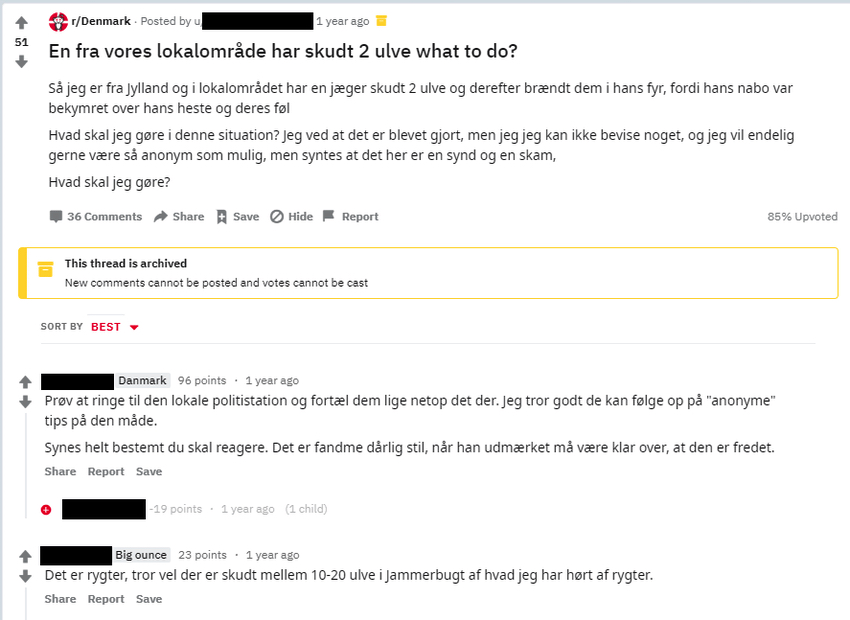
\includegraphics[width=\textwidth]{reddit}
\caption{Submission with comments \cite{reddit}}
\label{fig:reddit}
\end{figure}

The purpose of this chapter's analysis is to apply this existing literature and understanding of Russian methods of computational propaganda to the Reddit data (described in the introduction) with a focus on the Ukrainian crisis.
Reddit's content consists of submissions posted by users within subreddits (topical groups/communities); each submission may have replies (associated children comments), and each comment may have its own replies.
They form what is commonly called a ``thread'', or in formal terms, a ``tree'' because of its branches.
Figure \ref{fig:reddit} is an example submission with comments.

\begin{figure}[!ht]
\centering
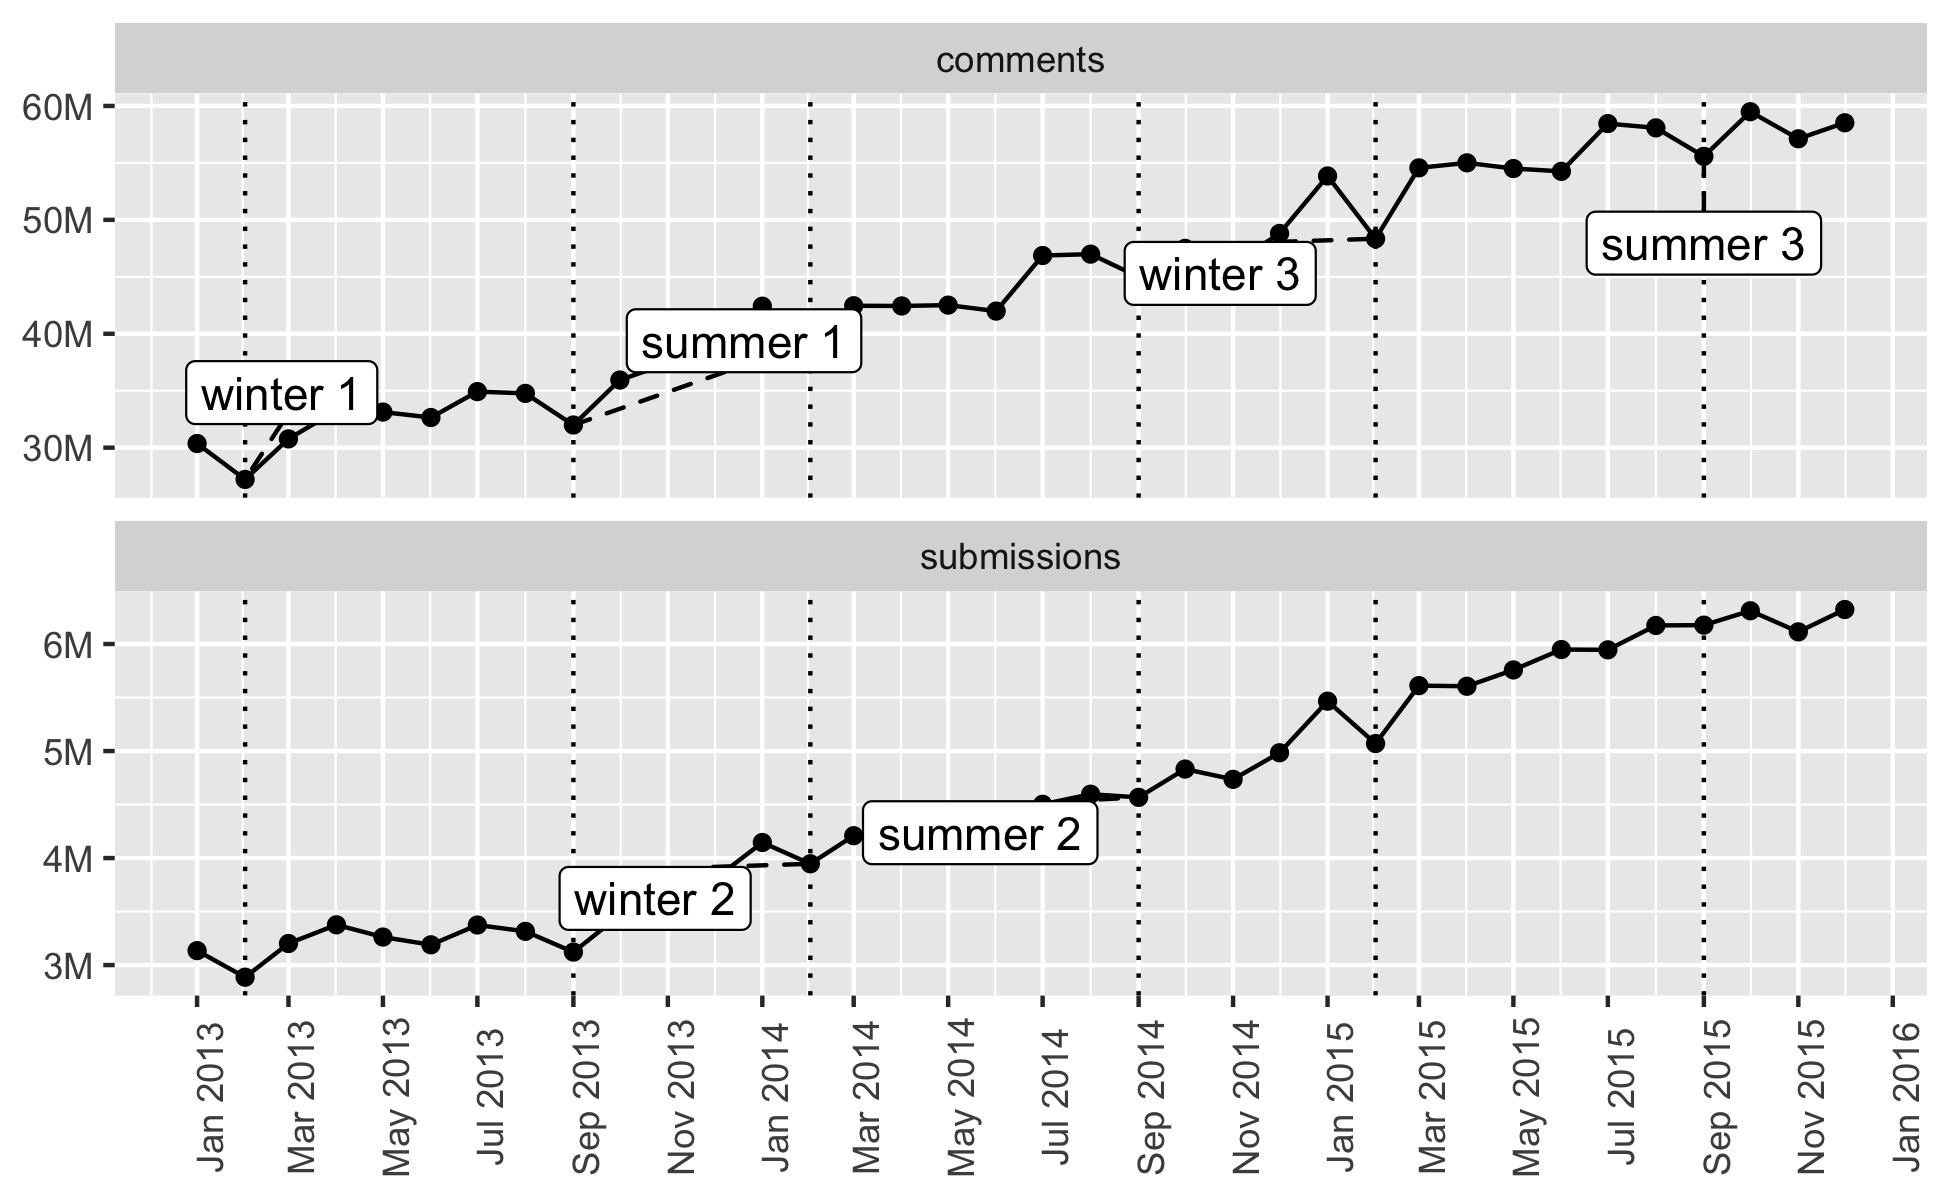
\includegraphics[width=\textwidth]{rus/count}
\caption{Comments and submissions}
\label{fig:count}
\end{figure}

The base dataset contains all 1,764,821,061 items or 163,041,230 submissions and 1,601,\\779,831 comments by 18,236,653 users across 460,025 subreddits on Reddit from January 2013 to December 2015.
These are freely available via Reddit's API, instead of downloading them ourselves, we use PushShift's archive which provides the very large dataset in an optimal compression format and has been used by other academic research \cite{pushshift}.
Figure \ref{fig:count} displays comments and submissions by month.

Though the most important events of the crisis start in late 2013 and end in  early 2015, the wider date range is selected to provide a control and context to capture change over time.
The total number of submissions and comments increases linearly each month, reflecting Reddit's growing popularity; in January 2013 there were 3,134,862 submissions and 30,365,867 comments, in December 2015 there were 6,322,479 submissions and 58,523,312 comments, increases of 101.68\% and 92.73\%.
The number of submissions and comments are directly correlated; over the three year period, the ratio of submissions to comments is never less than 9.42\% or greater than 11.11\%.

The most obvious pattern is a regular dip in activity at the end of each summer (September) and in winter (February).
Reddit's demographics skew younger such that this is probably connected to students returning to school after breaks.
This ``Eternal September'' has been recognized for decades.
Prior to the creation and adoption of the web, the Internet was used and populated by a much narrower range of people, usually professionals and experts at universities or self-selected early adopters and enthusiasts.
Usenet was a standard protocol which allowed users to send and receive messages in a format similar to Reddit; because new university students unfamiliar with norms gained access every year, September came to be dreaded by regular Internet users.
When AOL started offering consumer Usenet access in 1994, the previous September was said to have never ended \cite[p. 401]{isaacson2014}.

Next, the text component of each item (title and selftext for submissions, body for comments), is processed using the Python library spaCy. \footnote{The items, already divided into submissions and comments and split by month are downloaded from PushShift, decompressed into JSON, and saved into a format (Parquet) more appropriate for data work, split up by day.
The data include fields that are unnecessary for this research; for submissions only the id, created\_utc, edited, retrieved\_on, author, subreddit, url, title, and selftext fields are kept, for comments the id, created\_utc, edited, retrieved\_on, author, subreddit, link\_id, parent\_id, and body fields are kept.}
This natural language processing (NLP) toolkit uses modern techniques to correctly split (tokenize and parse) text in various languages into words, sentences, and other linguistic parts.
It also importantly converts words into vectors (lists, arrays, sequences) of numbers that are useful for computation and analysis, the basis of machine learning.

\begin{figure}[!ht]
\centering
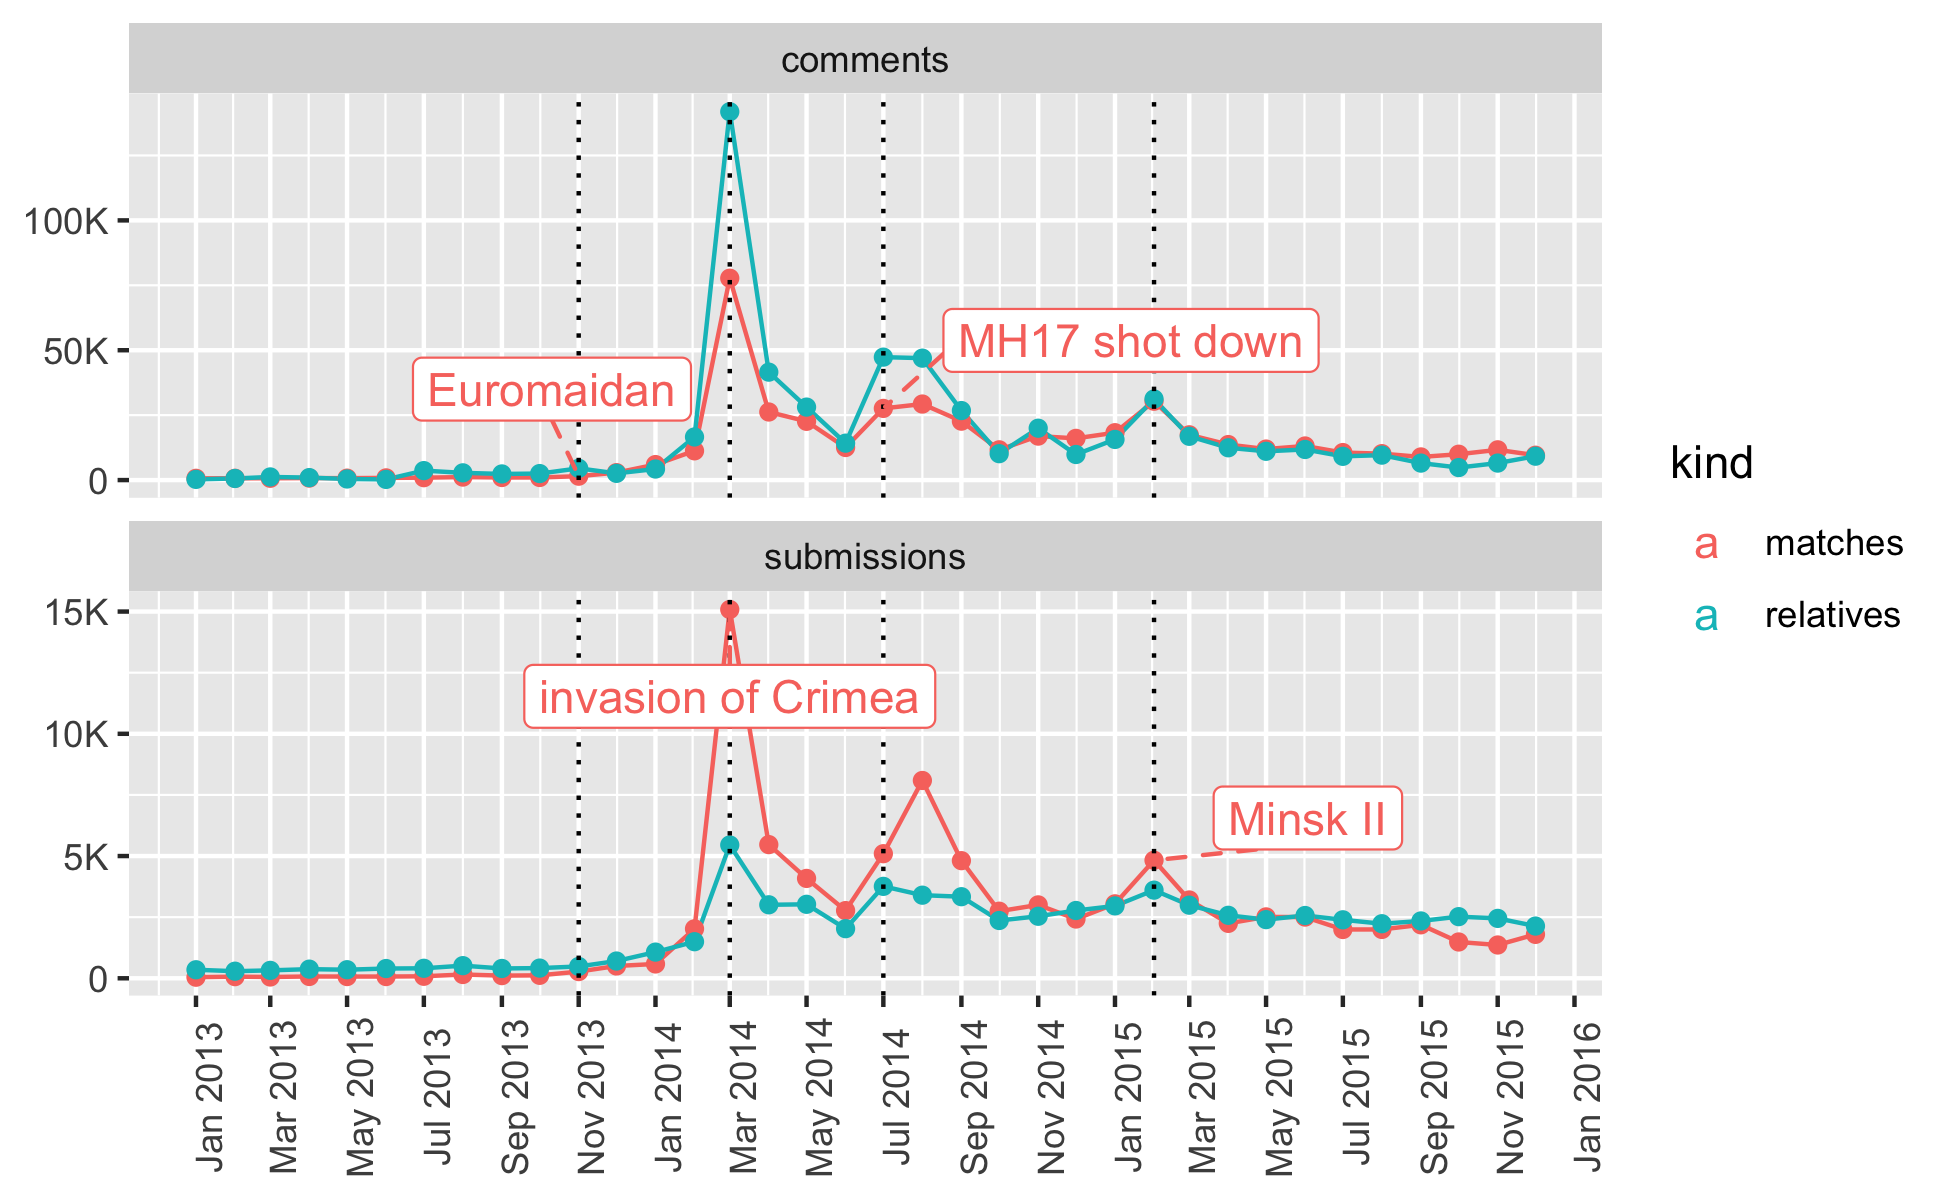
\includegraphics[width=\textwidth]{rus/things1}
\caption{Matches and relatives}
\label{fig:matches}
\end{figure}

The majority of items are irrelevant to the topic so the text of each item is filtered through a set of keywords and terms (case-insensitive).
The item is considered a ``match'' if ``Euromaidan'' or ``Donbas(s)'' are present, or if various combinations of ``Crimea'', ``Crimean(s)'', ``Putin'', ``Russia'', ``Russian(s)'', ``Ukraine'', ``Ukrainian(s)'', and terms related to ``annexation'' and ``invasion'' are found. \footnote{We only match against case-insensitive terms, an improvement would be to match against stems (used later in the chapter).}
In addition to these ``matches'', items connected to them are marked as ``relatives''.
For submissions, this includes every comment in response to it, for comments, this includes the submission the comment is in response to as well as any comments (children) replying to the match and the replies to those replies, etc.
Figure \ref{fig:matches} displays matches and relatives by month.

Euromaidan is a very unique term specific to the conflict and the Donbass region not commonly mentioned in Western popular media outside of the conflict
The dyads ensure we match on content including both countries or relevant topics (Putin, invasion) within the context of Russia, Ukraine, and Crimea.
Despite explicitly matching on Euromaidan, there is not a substantial increase in activity during that time (November 2013); that month there are 274 matched, 484 related submissions and 1,489 matched, 6,023 related comments.
Only in February 2014, the start of the invasion of Crimea, does there begin to be more matched than related submissions; this suggests that until this time it was a background topic brought up while discussing other primary topics.
Even then there are only 2,024 matched and 1,496 related submissions.
March 2014 follows with the peak of discussion: there are 15,084 matched, 5,453 related submissions, and 77,741 matched, 219,586 related comments, increases of 483.44\% for the submissions and 659.58\% for the comments.
The second peak of the comments is July 2014, the month of MH17's downing, with matched submissions rising the next month, even though ``MH17'' is not explicitly matched as a keyword.
February of 2015 is a third peak which is when the Minsk II ceasefire was signed, after that discussion returns to a similar level as in February 2014.
In total there are 86,969 matched, 70,447 related submissions and 459,053 matched, 1,033,697 related comments across the three years.
These patterns show that there are definite spikes and dips directly connected to the major events of the conflict and that our match terms are finding this relevant information.

\begin{table}[!ht]
\centering
\caption{Subreddits}
\begin{tabular}{lrrrrr}
\toprule
subreddit & \% & matches* & items & match \% & users \\
\midrule
worldnews             &   26.42 &   8643307 &    11747329 &    73.58 &   670840 \\
ukraine               &   10.39 &   3398449 &     4449535 &    76.38 &   226133 \\
UkrainianConflict     &    4.60 &   1504119 &     1765260 &    85.21 &   111672 \\
UkraineWarVideoReport &    3.46 &   1133154 &     1554034 &    72.92 &   125078 \\
CombatFootage         &    3.08 &   1007114 &     1543356 &    65.25 &   105349 \\
europe                &    2.22 &    725743 &     1857161 &    39.08 &    65027 \\
interestingasfuck     &    2.16 &    706541 &     4724053 &    14.96 &   218316 \\ß
news                  &    1.50 &    490912 &     5105814 &     9.61 &   102269 \\
politics              &    1.49 &    488251 &     6034055 &     8.09 &   111127 \\
AskARussian           &    1.46 &    476317 &      645065 &    73.84 &    25777 \\
conspiracy            &    1.40 &    458934 &     4302073 &    10.67 &    49986 \\
PublicFreakout        &    1.14 &    371466 &     5078293 &     7.31 &   106408 \\
neoliberal            &    1.09 &    355758 &     2846818 &    12.50 &    12885 \\
Damnthatsinteresting  &    1.06 &    348223 &     3066770 &    11.35 &   137484 \\
RussiaUkraineWar2022  &    0.82 &    269498 &      353670 &    76.20 &    35129 \\
ukpolitics            &    0.78 &    253829 &     1164034 &    21.81 &    10976 \\
NonCredibleDefense    &    0.69 &    226047 &      903671 &    25.01 &    21413 \\
nextfuckinglevel      &    0.65 &    211148 &     2937907 &     7.19 &    93475 \\
de                    &    0.62 &    201494 &     1500742 &    13.43 &    11344 \\
CryptoCurrency        &    0.55 &    181134 &     4980486 &     3.64 &    30981 \\
AskReddit             &    0.55 &    179205 &    39669986 &     0.45 &    56466 \\
ThatsInsane           &    0.51 &    168041 &     1069685 &    15.71 &    69375 \\
wallstreetbets        &    0.51 &    167041 &     7255226 &     2.30 &    46690 \\
Conservative          &    0.42 &    137499 &     1615715 &     8.51 &    19408 \\
CredibleDefense       &    0.34 &    112541 &      127050 &    88.58 &     6494 \\
russia                &    0.33 &    109417 &      171355 &    63.85 &    11906 \\
MapPorn               &    0.28 &     93019 &     1058404 &     8.79 &    32329 \\
canada                &    0.27 &     88474 &     1916732 &     4.62 &    16165 \\
CrazyFuckingVideos    &    0.26 &     85168 &     1691437 &     5.04 &    35943 \\
UkraineInvasionVideos &    0.26 &     84348 &      115132 &    73.26 &    13433 \\
summary (top 30)      &   69.32 &  22676191 &   121250848 &    32.64 &          \\
summary (all)         &  100.00 &  32713731 &  1456280549 &     0.49 &  2565090 \\
\bottomrule
\end{tabular}

\label{fig:subreddits}
\end{table}

These results are expected if the keyword filtering is correctly matching relevant data.
However, Reddit is divided into subreddits, which means that we can further remove large chunks of unrelated topics.
A common issue with social science datasets is sports can cause false positives; every four years in the World Cup or Olympics, countries ``battle'' countries and teams and fans ``invade'' the other team's stadium.
The World Cup semi-final between Brazil and Germany in 2014, games between Ukraine and Russia, or interactions between athletes from these countries have usually have limited connection to world politics.
Similarly, Reddit's demographics tend towards many discussions about videogames and e-sports, both of which are international interests.
Other topics are generally irrelevant to this research.
Therefore, out of the original set with at least 100 matches and relatives, 69 subreddits and their matches and relatives, including r/soccer, r/hockey, r/eurovision, r/languagelearning, and r/starcraft are excluded.
Table \ref{fig:subreddits} displays the 30 subreddits with the most matches and relatives.

There are total 1,560,766 matches and relatives by 193,560 users across 5,138 subreddits.
The r/worldnews subreddit accounts for 42.2\% of all matches and relatives, though only 3.48\% of all items in that subreddit are matches or relatives, slightly below the average mean of 4.8\% for the top 30.
The top 7 subreddits account for more than 73\% of all matches and relatives, and the top 30, 85.71\%. \footnote{This is a standard power law distribution, discussed later in this chapter.}
Only a few subreddits have to be targeted to monitor and direct these discussions and the Reddit homepage has and still does link to r/worldnews, directing users to it.
r/worldnews has the most unique users (85,829) in these discussions, only two other subreddits have more than 20,000 users, and r/russia has 4,578, r/ukraine 3,080, and r/conspiracy 3,875. 
It would take small numbers of users (real or not) to dominate these discussions, especially if we assume that the average user is not coordinating with others to push a narrative.
Finally, four subreddits have double-digit match rates, three: r/UkrainianConflict (37.56\%), r/russia (20.5\%), r/ukraine (46.16\%) have match rates over 20\%.

\subsection{Classification}

We need some way of detecting Russian propaganda and the users that post it.
There are many ways to categorize textual content and by extension the producers of that content.
These range from the relatively unsophisticated but time-tested manual coding of documents to an ever-expanding set of modern techniques.
The rise of machine learning has brought many supervised and unsupervised systems into play including naive Bayes classifiers, support vector machines, neural networks, and various natural language processing approaches.
Woolley and Guilbeault's analysis of the 2016 US presidential election via Twitter used BotOrNot, a software suite which takes into account a wide array of features to aid in bot detection \cite[p. 198]{woolley2018}.

These approaches all have strengths and weaknesses relative to a given dataset though many options would work fine for this particular study.
Our chosen method is based on a few specific goals.
While heavily influenced and modeled after Woolley and Guilbeault, this research not is particularly concerned whether a user is a ``bot'' or ``troll'', setting aside the muddled use of those terms.
The abundance of features these software suites take into account can be detrimental as they are highly specific, sensitive to the changing behavior of users constantly trying to avoid detection, and difficult to describe or justify to a non-technical audience.

Our intended audience is not just computer scientists or machine learning experts but political and other social scientists as well as a non-academic audience.
If the author fails to understand the complexities or nuances of neural networks or fails to impart that knowledge to the reader then confidence in the overall argument is lost.
Therefore, in classification and in each step of this research simple and pragmatic techniques are favored as they are easier to describe, defend, and debug.

For text and user classification we use an approach based on web addresses or URLs.
Google rose to prominence and profitability in the early 2000s thanks to their PageRank system which categorizes and ranks sites based on which sites in turn reference or link to them.
This was inspired by the custom of citations and references that powers academic research \cite[p. 462]{isaacson2014}.
To cite an author or work is to if not agree with them to at the very least acknowledge that said work has some kind of social currency; it is a form of provenance.

Web addresses themselves, not just the resources they reference, are often packed with information including the date, author, or title.
They always include a domain address, which is registred with in public information about the owner.
Given the assumption that individuals generally spread material that they agree with, by categorizing domains we can more broadly categorize content and the users that link to this content.
For example, \url{www.nytimes.com/2020/08/05/us/politics/state-department-russian-disinformation.html}.

\begin{table}[!ht]
\centering
\caption{Cites}
\begin{tabular}{lrrrrrr}
\toprule
{} & \% & cites & users &  cites / & \% prog & \% cons \\
domain &  &  &  & users & users & users \\
\midrule
reddit.com*           &   21.94 &   2722645 &   630963 &         4.32 &         13.41 &          9.79 \\
youtube.com*          &    9.62 &   1193237 &   251651 &         4.74 &         16.49 &         17.00 \\
imgur.com             &    6.01 &    746031 &   200126 &         3.73 &         10.76 &          9.57 \\
wikipedia.org         &    3.70 &    459470 &   126526 &         3.63 &         19.83 &         11.21 \\
twitter.com*          &    3.45 &    428391 &    81020 &         5.29 &         23.65 &         22.73 \\
washingtonpost.com    &    2.03 &    252175 &    68845 &         3.66 &         40.00 &         19.00 \\
nytimes.com*          &    1.37 &    170305 &    54124 &         3.15 &         32.52 &         16.96 \\
cnn.com               &    1.13 &    139847 &    47536 &         2.94 &         36.94 &         22.44 \\
archive.org*          &    1.06 &    131008 &    20095 &         6.52 &         29.30 &         37.80 \\
google.com*           &    1.05 &    130314 &    48537 &         2.68 &         16.23 &          9.06 \\
politico.com          &    0.97 &    120307 &    37074 &         3.25 &         45.09 &         26.10 \\
thehill.com           &    0.90 &    111112 &    30702 &         3.62 &         43.44 &         28.39 \\
theguardian.com       &    0.84 &    103685 &    39020 &         2.66 &         41.09 &         17.61 \\
huffingtonpost.com*   &    0.72 &     89205 &    32861 &         2.71 &         44.03 &         18.67 \\
sli.mg                &    0.72 &     88865 &    15886 &         5.59 &         10.85 &         22.45 \\
independent.co.uk     &    0.62 &     77328 &    22716 &         3.40 &         44.67 &         13.21 \\
reuters.com           &    0.56 &     69324 &    23100 &         3.00 &         36.07 &         23.85 \\
wikileaks.org         &    0.52 &     64918 &    12213 &         5.32 &         19.71 &         23.63 \\
breitbart.com         &    0.50 &     62530 &    17220 &         3.63 &         25.17 &         52.35 \\
politifact.com        &    0.49 &     60982 &    26742 &         2.28 &         32.46 &         13.41 \\
foxnews.com           &    0.46 &     57092 &    23051 &         2.48 &         24.60 &         35.29 \\
bbc.com*              &    0.43 &     53800 &    24014 &         2.24 &         22.17 &         17.11 \\
businessinsider.com   &    0.41 &     51133 &    24106 &         2.12 &         34.92 &         21.58 \\
fivethirtyeight.com   &    0.38 &     47223 &    18570 &         2.54 &         39.89 &         11.51 \\
facebook.com*         &    0.37 &     46391 &    18790 &         2.47 &         18.70 &         10.88 \\
nbcnews.com           &    0.37 &     46260 &    19792 &         2.34 &         42.94 &         20.70 \\
realclearpolitics.com &    0.34 &     42197 &    15416 &         2.74 &         34.86 &         20.09 \\
theatlantic.com       &    0.34 &     41577 &    19370 &         2.15 &         44.51 &         17.66 \\
go.com                &    0.33 &     41301 &    17435 &         2.37 &         44.54 &         17.30 \\
npr.org               &    0.31 &     38915 &    18260 &         2.13 &         43.26 &         13.57 \\
summary (top 30)      &   61.96 &   7687568 &          &         3.32 &         31.07 &         20.03 \\
summary (all)         &  100.00 &  11761790 &  1174637 &         1.97 &         45.13 &         41.51 \\
\bottomrule
\end{tabular}

\label{tab:doms}
\end{table}

This url contains a date, title, and topic (US politics), and is hosted on the New York Times (nytimes.com) domain.
We obtain all the domains in the dataset by extracting the url in each submission as well as those found in the body text of submissions and comments, using the already processed spaCy data.
Domains are then extracted from addresses, careful to take into account the variety of international suffixes including .co.uk. \footnote{Technically, the ``public suffix'' of the domain is captured using the publicsuffix2 Python library.}

The 30 most cited-domains are summarized in Table \ref{tab:doms}.
Domains from the previously excluded subreddits are not included, and we further filter the dataset by removing 8 users that are apparent bots, including u/AutoModerator and u/autotldr (an article summarizer), common across subreddits, and u/ModeratorLog and u/PoliticBot, which mirror other subreddits.
We also merge several related domains and ``link shorteners'' together; reddit.com and redd.it are different names for the same thing.

The distribution is top-heavy with 313,409 of 426,426 (68.61\%) citations distributed among these 30 domains submitted by 84,735 of 149,365 (56.73\%) users.
Wikipedia is the most cited, with 92,254 or 20.14\% of all cites despite being editable by anyone, prone to opaque conflicts between editors, and having been the target of multiple attempts by individuals, organizations, and state entities to whitewash reputations \cite{wiki:criticism}.
This tracks with the expectation of ``facts'' and evidence in the Russian blogosphere, a reaction to unreliable state media \cite[p. 25]{woolley2018}.
Wider Soviet and Russian disinformation has emphasized evidence, but it is not obvious whether this use of Wikipedia is a Redditism or widely-used elsewhere.

Reddit is another 18.40\% of cites; between it, Wikipedia, imgur.com, YouTube, and Twitter are more than 53.58\% of all links.
Facebook only has 1,509 cites, reflecting its parallel ``walled garden'' environment of personal connections.
The news sources themselves are distributed evenly across various regions with media in the UK (theguardian.com, bbc.com, telegraph.co.uk, dailymail.co.uk, independent.co.uk) and US (nytimes.com, washingtonpost.com, cnn.com, bloomberg.com, wsj.com) well-represented.
Ukrainian \\ (kyivpost.com) and independent Russian outlets are present (themoscowtimes.com) as well as aljazeera.com and globalresearch.ca.
Perhaps most notable are the multiple outlets owned, sponsored, or controlled by the Russian government: itar-tass.com, rt.com, and ria.ru.
Similarly, rferl.org, Radio Free Europe/Radio Liberty, is funded by the US government.
These Russian state domains are the basis of our categorization scheme.

We begin with a ``core'' list of 14 Russian government-owned or controlled domains including the official Kremlin site (kremlin.ru), Ministry of Defense site (mid.ru), and major domestic media providers (russia.tv, 1tv.ru, voiceofrussia.com).
To these are added domains controlled by the Iranian and Chinese governments: Press TV, Fars News, Xinhuanet, and China Daily.
These domains are all selected based on their presence within the dataset.
Our core assumption is that state media is unlikely to publish anything but state propaganda, or at the very least will not publish content contrary to the interests of the state.
If a user cites these sources often they are spreading, willingly or not, propaganda.

While all have government ties, they have different origins.
Rossiyskaya Gazeta (rg.ru) came into being in 1990 just before the fall of the USSR \cite{strovsky2021}.
Russia-24 (vesti.ru) and RT were founded during the Putin era \cite[p. 305]{yablokov2015}.
ITAR-TASS and RIA Novosti are much older, the former began in 1904 under the tsarist regime and continued into the Soviet era through today, and the latter was established in 1941 \cite{watanabe2017, simons2016}.
They are supplemented by a number of publications that while not officially government-owned have close ties and loyalties to the Kremlin, often through the convoluted system of oligarchs.
Izvestia (iz.ru) was founded in 1917 during the revolution and is today owned by Yuriy Kovalchuk's National Media Group; Kovalchuk is known as ``Putin's banker'' \cite{voltmer2000}.

These unofficially Kremlin-aligned sites are contained in a separate ``extended'' list with publications which have been appropriated; lenta.ru saw mass firings and resignations by the editorial staff in early 2014 in a shift towards propaganda \cite[p. 45]{lazitski2020}.
There are also a number of sites with hidden ties that are repeaters of the state line including Global Research (globalresearch.ca) and New Eastern Outlook (journal-neo.org); according to the US State Department, NEO presents itself as an academic journal \cite{nyt:globalresearch, statedept}.

We count domains with extremist anti-Semitic and conspiracy theorist views among the extended grouping.
Russia, like many other countries, has a troubled history of Jewish relations. 
When the surrounding countries divided up the Poland-Lithuanian Commonwealth at the end of the 18th century, the large population of Jews ended up Russian subjects (not citizens, not Russians), restricted to the Pale of Settlement in the west; in the late 19th and early 20th century there were numerous pogroms (mass violence) against these Jewish communities, this led to mass emigration to the United States and other countries.
In the early 1950s, at the height of his power, Stalin's prejudices and paranoias ended with him giving support to the arrest and torture of dozens of doctors in the medical community in a supposed Jewish ``Doctors' plot''; the media blitz of the Russian state media and the prosecution of the non-existent conspiracy stopped with his death in March 1953 \cite[ch. 56]{montefiore2007}.
Putin has used similar rhetoric, suggesting Jews (or Ukrainians or Tartars with Russian citizenship) were responsible for meddling in the 2016 presidential election in the US \cite{putin2018}.
Violence and rhetoric against Jews has increased in the US in recent years with the infamous ``tiki torch'' parade in Charlottesville in 2017, attacks in Pittsburgh in 2018, Poway, California and Jersey City in 2019, and numerous smaller incidents like the taking of hostages at a synagogue in Colleyville, Texas in 2022. 
The Unz Review (unz.com) and Russia Insider (russian-insider.org) engage in Holocaust denial and anti-Semitic stances along with generally favorable coverage of Russia \cite{bevensee2018}.

This anti-Semitic content often overlaps with conspiracy theories and can be found on the political extremes.
One dominant notion is that of false flags where (usually) the United States government is said to engage in covert actions against its own citizenry to allow for increased control or military engagement, the primary example being the 9/11 truther movement.
Starting with the claims of ``crisis actors'' in the Sandy Hook school shootings in 2012, it is perhaps difficult to find events of mass violence not claimed to be fake.
Conspiracy theories are well-represented in Alex Jones-owned domains: InfoWars (infowars.com) and PrisonPlanet (prisonplanet.com).
Jones has made numerous claims of false flags and in 2022 was ordered to pay \$45.2 million in punitive damages to the parents of a victim of Sandy Hook \cite{jones2022}.

The basis and probable cause of many of these claims is due to US military action.
Veterans Today (veteranstoday.com) explicitly targets former US service members with a pro-Russian message and was partners with NEO \cite[p. 24]{statedept}..
We include a number of domains in the extended list for content which while critical and skeptical of neoliberal US foreign policy, fails to apply that same skepticism to Russian intentions, in some cases parroting Kremlin-associated material.
On the right of the political spectrum are sites favorable to former Republican presidential candidate and long-time libertarian Ron Paul: Ron Paul Institute (ronpaulinstitute.org) and The Daily Bell (thedailybell.com).
The left is represented by OpEdNews (opednews.com) and Antiwar.com.
This kind of selectivity critical reporting is reminiscent of Western liberals like Walter Duranty, former Moscow Bureau Chief of the New York Times.
Despite winning a Pulitzer for favorable reporting on the USSR in the early 1930s, at the same time he repeatedly denied the famine in Ukraine known as the Holodomor \cite[p. 445]{dutton2005}.

\begin{table}[!ht]
\centering
\caption{Rus domains}
\begin{tabular}{rlrrrrr}
\toprule
rank & domain &       \% &  cites &  users &  cites/users &  \% rus users \\
\midrule
9                &                         rt.com &   27.07 &   5425 &   2070 &         2.62 &        43.91 \\
16               &                 itar-tass.com* &   10.21 &   2046 &    624 &         3.28 &        63.83 \\
25               &                         ria.ru &    6.35 &   1272 &    513 &         2.48 &        51.65 \\
27               &              globalresearch.ca &    6.18 &   1238 &    625 &         1.98 &        37.72 \\
30               &                  zerohedge.com &    5.74 &   1150 &    458 &         2.51 &        51.30 \\
34               &                sputniknews.com &    5.40 &   1082 &    382 &         2.83 &        61.37 \\
52               &            ian56.blogspot.com* &    3.30 &    661 &      6 &       110.17 &        98.49 \\
57               &             russia-insider.com &    3.04 &    610 &    141 &         4.33 &        77.21 \\
66               &              voiceofrussia.com &    2.61 &    523 &    242 &         2.16 &        45.89 \\
67               &                       lenta.ru &    2.60 &    521 &    194 &         2.69 &        55.28 \\
92               &                      pravda.ru &    1.88 &    377 &    181 &         2.08 &        53.32 \\
102              &                     kremlin.ru &    1.66 &    332 &    162 &         2.05 &        48.49 \\
103              &                    antiwar.com &    1.65 &    331 &     92 &         3.60 &        76.44 \\
108              &                       rbth.com &    1.55 &    311 &    132 &         2.36 &        58.84 \\
128              &            washingtonsblog.com &    1.26 &    253 &    110 &         2.30 &        59.68 \\
145              &                   infowars.com &    1.07 &    215 &     86 &         2.50 &        54.88 \\
153              &  informationclearinghouse.info &    1.04 &    208 &     98 &         2.12 &        61.06 \\
156              &                      gazeta.ru &    1.00 &    201 &    132 &         1.52 &        36.32 \\
165              &                     presstv.ir &    0.93 &    187 &    123 &         1.52 &        34.76 \\
169              &                     ukraina.ru &    0.91 &    183 &     16 &        11.44 &        90.71 \\
181              &                       sott.net &    0.85 &    170 &     75 &         2.27 &        65.29 \\
193              &                    rusvesna.su &    0.79 &    159 &     83 &         1.92 &        47.17 \\
196              &                    lifenews.ru &    0.78 &    156 &     93 &         1.68 &        46.15 \\
203              &                voltairenet.org &    0.73 &    146 &     71 &         2.06 &        53.42 \\
207              &                  xinhuanet.com &    0.72 &    144 &     91 &         1.58 &        45.83 \\
214              &                       vesti.ru &    0.68 &    137 &     84 &         1.63 &        35.77 \\
216              &                         mid.ru &    0.68 &    136 &     64 &         2.12 &        57.35 \\
227              &           paulcraigroberts.org &    0.64 &    128 &     61 &         2.10 &        53.91 \\
235              &           ronpaulinstitute.org &    0.61 &    122 &     55 &         2.22 &        43.44 \\
280              &              beforeitsnews.com &    0.48 &     96 &     57 &         1.68 &        23.96 \\
& summary (top 30) &   92.40 &  18520 &   7121 &         6.19 &        54.45 \\
& summary (all)    &  100.00 &  20043 &   7853 &         4.30 &        58.11 \\
\bottomrule
\end{tabular}

\label{tab:rus_doms}
\end{table}

Of course, any categorization based on site content alone is subjective.
This arbitrariness is one of the criticisms leveled at other compilation attempts of pro-Russian sources like PropOrNot \cite{chen2016}.
Importantly, all domains included in the extended list have a higher percentage of citations from ``rus users'' that post these pro-Russian domains, core and extended.
For example, of all citations of nytimes.com, 21.05\% are from users that have cited these selected domains at least 10 times over the three-year period in the original dataset.
In comparison, russia-insider.com is at 77.21\% and ronpaulinstitute.org is at 43.44\%; of the 30 most-cited domains in Table \ref{tab:doms} (average 26.59\%), 18 have rates below 25\%, but of the 30 most-cited domains from the core and extended set (average 54.45\%), only 4 are below 40\%.
We assume that individuals will cite material which they not only agree with but which generally agrees with other material they have posted.
Since users have the ability to delete accounts on Reddit, in order to not overcount cites by rus users, we remove the specially marked ``[deleted]'' user.
Table \ref{tab:rus_doms} displays summary stats for the rus domains.

This list is top-heavy with 92.40\% of all citations of pro-Russian domains; the 3 most-cited (itar-tass.com, rt.com, ria.ru) are from the core set and are a combined 43.63\% of cites, they are ranked 9th, 16th, and 25th of all links posted about this topic.
The first domain not from the core set is globalresearch.ca (ranked 27th overall) with content from Jones, Unz, and numerous other conspiracy-focused entities.
37.72\% of all users that post it are ``rus'', compared to 43.91\%, 63.83\%, and 51.65\% of the first 3 and the overall mean of 58.11\%.
It also is the only of the first 17 rus domains with fewer than 2 cites per user; this suggests organic activity.

The sum activity is small; domains from the rus core and extended lists total 
20,043 cites by 7,853 users, 4.70\% of 426,426 total cites across all domains.
Of the rus set, rt.com is cited by the most users (2,070), ian56.blogspot.com by 6; ``Ian56'' is a known Russian troll across social networks \cite[p. 278]{heffer2020}.
Of 331 cites by 92 users of antiwar.com, 76.44\% were by rus users.
These numbers suggest that a very limited set of users are responsible for most of the ideological content on this topic, pro-Russians posting antiwar content is framing that is only obvious when those cites are aggregated.

Finally, the presence of Paul Craig Roberts' site is worth noting.
Assistant Treasury Secretary during the Reagan administration, he has since become a writer for unz.com, has been featured on RT as a guest, is a 9/11 ``Truther'', argued for Holocaust denialism and other conspiracy theories, and was accused of ``Putin worship'' \cite[p. 2388]{marmura2014}.
He is an example of a small but prominent group of individuals and institutions which favor and legitimatize each other.

\begin{table}[!ht]
\small
\centering
\caption{Wiki articles}
\begin{tabular}{lrrrrr}
\toprule
{} &       \% &  cites &  users &  cites/ & \% rus \\
wikipedia.com/wiki/                                               &         &        &        & users & users             \\
\midrule
Ukraine                                            &   10.92 &   1056 &     90 &        11.73 &         1.80 \\
Budapest\_Memorandum\_On\_Security\_Assurances         &    5.97 &    577 &    425 &         1.36 &         6.59 \\
Holodomor                                          &    5.35 &    517 &    312 &         1.66 &         4.64 \\
Crimea                                             &    4.97 &    481 &    179 &         2.69 &         5.41 \\
Euromaidan                                         &    4.11 &    397 &    152 &         2.61 &        14.36 \\
2014\_Crimean\_Crisis                                &    3.36 &    325 &     48 &         6.77 &        14.77 \\
Crimean\_Status\_Referendum,\_2014                    &    3.29 &    318 &    176 &         1.81 &        15.09 \\
Covert\_United\_States\_Foreign\_Regime\_Change\_Actions &    3.16 &    306 &    173 &         1.77 &        30.72 \\
Whataboutism                                       &    2.69 &    260 &    168 &         1.55 &        11.15 \\
Nuclear\_Weapons\_And\_Ukraine                        &    2.42 &    234 &    115 &         2.03 &         3.42 \\
Iran\_Air\_Flight\_655                                &    2.13 &    206 &    161 &         1.28 &         4.37 \\
2014\_Ukrainian\_Revolution                          &    2.05 &    198 &     73 &         2.71 &         9.09 \\
Russo-Georgian\_War                                 &    1.87 &    181 &    136 &         1.33 &        14.92 \\
Viktor\_Yanukovych                                  &    1.86 &    180 &     61 &         2.95 &         2.78 \\
Annexation\_Of\_Crimea\_By\_The\_Russian\_Federation     &    1.86 &    180 &     89 &         2.02 &         3.89 \\
Ukrainian\_Insurgent\_Army                           &    1.59 &    154 &     86 &         1.79 &         9.74 \\
Siberia\_Airlines\_Flight\_1812                       &    1.59 &    154 &    125 &         1.23 &        10.39 \\
Crimean\_Referendum,\_1994                           &    1.56 &    151 &     81 &         1.86 &        26.49 \\
Stepan\_Bandera                                     &    1.54 &    149 &     97 &         1.54 &        19.46 \\
Right\_Sector                                       &    1.50 &    145 &     87 &         1.67 &         8.28 \\
Svoboda\_(Political\_Party)                          &    1.47 &    142 &     93 &         1.53 &         5.63 \\
Deportation\_Of\_The\_Crimean\_Tatars                  &    1.44 &    139 &    109 &         1.28 &         9.35 \\
Crimean\_Tatars                                     &    1.44 &    139 &     56 &         2.48 &         2.88 \\
Massacres\_Of\_Poles\_In\_Volhynia\_And\_Eastern\_Galicia &    1.40 &    135 &     81 &         1.67 &        30.37 \\
2014\_Pro-Russian\_Unrest\_In\_Ukraine                 &    1.39 &    134 &     58 &         2.31 &         8.96 \\
Crimean\_War                                        &    1.39 &    134 &     76 &         1.76 &         4.48 \\
Igor\_Girkin                                        &    1.37 &    132 &     73 &         1.81 &        15.91 \\
Azov\_Battalion                                     &    1.30 &    126 &     85 &         1.48 &        20.63 \\
Tu\_Quoque                                          &    1.29 &    125 &     60 &         2.08 &         6.40 \\
Ukrainian\_Presidential\_Election,\_2010              &    1.23 &    119 &     68 &         1.75 &        13.45 \\
summary (top 30)                                   &   77.50 &   7494 &   3593 &         2.35 &        11.18 \\
summary (all)                                      &  100.00 &   9670 &   5126 &         1.93 &        11.34 \\
\bottomrule
\end{tabular}

\label{tab:wiki}
\end{table}

In the way these individuals and sources are telling points of reference, facts and events can serve the same purpose; we end this section with a review of commonly cited Wikipedia articles in Table \ref{tab:wiki}.
The sum activity is once again small, though Wikipedia was the most-cited domain, only 9,670 links by 5,126 users are extractable articles, of which the 30 most-cited account for 77.50\%.
Only 3 articles have more than 2.95 cites per user.
Pro-Russian users strongly favor certain topics and articles, those over the average of 11.34\% of rus users track Russian talking points.

The Budapest Memorandum (6.59\% rus users) was a multilateral agreement signed in 1994 which promised to respect the territorial integrity of Ukraine; multiple countries accused Russia of breaking this agreement with the invasion of Crimea.
Nuclear weapons and Ukraine may have a low rus cite percentage (3.42\%) because Ukraine surrendering their nuclear weapons to Russia was part of the deal.
The Holodomor (4.64\%) was the mass starvation of Ukrainians as a policy of the USSR in the early 1930s; the Crimean Tatars were (2.88\%) displaced over the centuries, faced Nazi atrocities, mass deportation during World War II due to alleged Nazi collaboration (9.35\%), then were banned from return until 1989.
The Tatars were an estimated 98\% of the population when Crimea was originally annexed in 1783, by 2004 that number was 12\%.

Covert Foreign regime change actions of the US has the highest rus percentage (30.72\%); the Russo-Georgian War (14.92\%) is oft-cited as an example of Western expansion into Russia's traditional sphere of influence.
Other apparent examples of whataboutism are attempts to tie the downing of MH17 to past downings of civilian planes.
Flight 655 was a downing by the USS Vincennes in 1988, Flight 1812 was a downing by Ukraine in 2001.
Igor Girkin (15.91\%) is a hard-line Russian nationalist, active in military actions throughout the conflict, former Supreme Commander of the self-proclaimed Russian ``Donetsk People's Republic'' accused of multiple atrocities including the downing of MH17.

One of the common talking points of Russian propaganda around the Ukrainian conflict is to paint the Ukrainian government as fascist and to associate it with Nazi actions in World War 2.
The Azov Battalion (20.63\% rus users) and Right Sector are far-right paramilitary groups operating in Ukraine against Russian interests.
Svoboda is an ultranationalist political party.
The volunteer battalion especially would become a feature of Russian propaganda, a justification for war in 2022 after it was reorganized and integrated into the Ukrainian National Guard in late 2014.
Stepan Bandera (19.46\%) was a fascist during World War 2 responsible for a number of atrocities, Putin has invoked him directly as a justification for Crimea's annexation: ``...saving them from the new Ukrainian leaders who are the ideological heirs of Bandera, Hitler's accomplice during World War II'' \cite[p. 204]{garcia2016}.
``Banderites'' and related terms are tells of Russian propaganda, he is not well-known in the US.
The Volhynia massacres (30.37\%) were carried out by the Ukrainian Insurgent Army, formed in October 1942 by Banderas' followers to fight Soviets and Nazis.

The multiple referenda are instructive.
Crimea has a majority Russian population as does much of southeastern Ukraine, in a state of insurgency since 2014.
Not surprisingly, referenda there tend to favor Russian interests, and the 2014 referendum in particular has been considered illegitimate by most countries due to Russian intervention.
The article for that year's referendum is cited by 16.09\% rus users, the 1994 version has the third-highest rus user percentage of 26.49\%.
These fit the confusing pattern of authoritarian regimes embracing democracy and popular will when convenient.

\begin{table}[!ht]
\centering
\caption{User groups}
\begin{tabular}{lrrrrrr}
\hline
& & & comment & comment & submission & submission \\
group & users & doms & matches & relatives & matches & relatives \\
\hline
neutral &  193647 &  346457 &           381264 &             776965 &               39312 &                 52842 \\
spreader &     262 &   80023 &            40618 &              52658 &               19011 &                  7143 \\
superspreader &      75 &   43239 &            13201 &              16223 &               13280 &                  3118 \\
totals &  193910 &  518141 &           459054 &            1033697 &               87008 &                 72688 \\
\hline
\end{tabular}

\label{tab:rus_groups}
\end{table}

Wikipedia articles are useful to provide context, but they are not included in either the core or extended list of Russian domains.
Using the combined list we are able to categorize users as shown in Table \ref{tab:rus_groups}.
Users that cite these domains at least 10 times over the three-year period of the dataset are considered ``spreaders'' of pro-Russian propaganda, with this limit used as a buffer to allow for unintentional activity.
Those that cite them 25 or more times are considered ``superspreaders''.
Too low of a cutoff will capture incidental posters or those that post a large and wide variety of material, too high of a cutoff removes the users we most want to capture, but these are arbitrary thresholds.
Without filtering subreddits, of the 193,910 users in the matched dataset, 193,647 (99.86\%) are neutral with fewer than 10 cites, 262 (0.14\%) are spreaders of pro-Russian content with at least 10 but less than 25 cites, and another 75 (0.04\%) are superspreaders with at least 25 cites. 
The totals include bots; the rest of the table shows pro-Russian users are a very small part of the dataset.

\subsection{Network Analysis}

With users categorized we can observe how they are distributed and how they interact using network analysis.
We want to know how the user network is shaped, whether pro-Russian users exist in their own isolated communities, or if they are ignored by others or receive many responses from a variety of people and therefore drive discussion.
Has Russian propaganda reached positions of influence within the core of the network?

Network analysis consists of statistical techniques that take into account features within networks (graphs) to determine their overall shape and layout. Graphs are composed of nodes (such as users) and their edges (connections). Graphs can be directed (displaying the flow of connections and information) or undirected (only showing that there is a connection).
Nodes have overall degree (the number of nodes which connect to them) and in the case of directed networks in-degree (incoming connections) and out-degree (outgoing connections) \cite[pp. 199-200]{woolley2018}.
There are many useful measures within graph theory but how useful those measures are and indeed the very basis of a graph is arbitrary and dependent upon the data and its interpretation.
It is up to the researcher to turn unstructured content into a truly representative model.
We use the NetworkX library, written in Python, to build and analyze our graphs.

\begin{figure}[!ht]
\centering
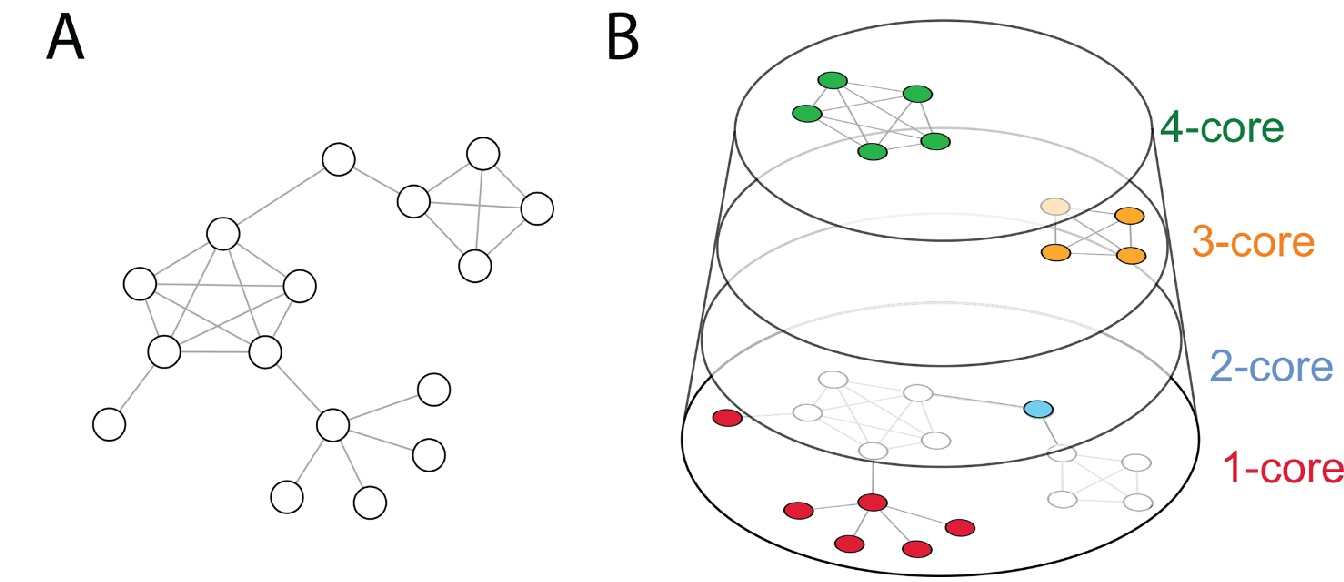
\includegraphics[width=\textwidth]{rus/kcore}
\caption{k-core \cite{barbera2015}}
\label{fig:kcore}
\end{figure}

Our first analysis consists of k-core decomposition.
This decomposition splits the largest-connected component of a network (subset of the network with the most connected nodes) into k-shells where each individual shell is composed of all nodes with the same or higher number of connections.
Specific cores contain multiple shells: the 10-core contains k-shells 1 through 10.
K-core decomposition is mostly dependent upon a node's degrees.
Nodes located in the highest shells have the most connections and are most able to disseminate information through the network and nodes in the lower shells are on the periphery \cite[p. 200]{woolley2018}.
Figure \ref{fig:kcore} illustrates the k-core for a random graph.

To reiterate, the structure of many graphs is arbitrary.
The same data can be represented in a graph that connects different nodes using different criteria, is directed or undirected, or has different weights measuring the strength of connections between nodes.
Woolley and Guilbeault base their k-core analysis on a network of Twitter users where connected users have both retweeted each other \cite[p. 202]{woolley2018}.
In order to capture the strictest measure of connection, our k-core analysis is run on an undirected network where nodes (users) have any edge (tie) only if they have posted in response (directly or to a child reply) to each other at least once.
We want to capture users that are interacting, not just those that post a lot of content (spam) but are ignored by the rest of the network.

\begin{figure}[!ht]
\centering
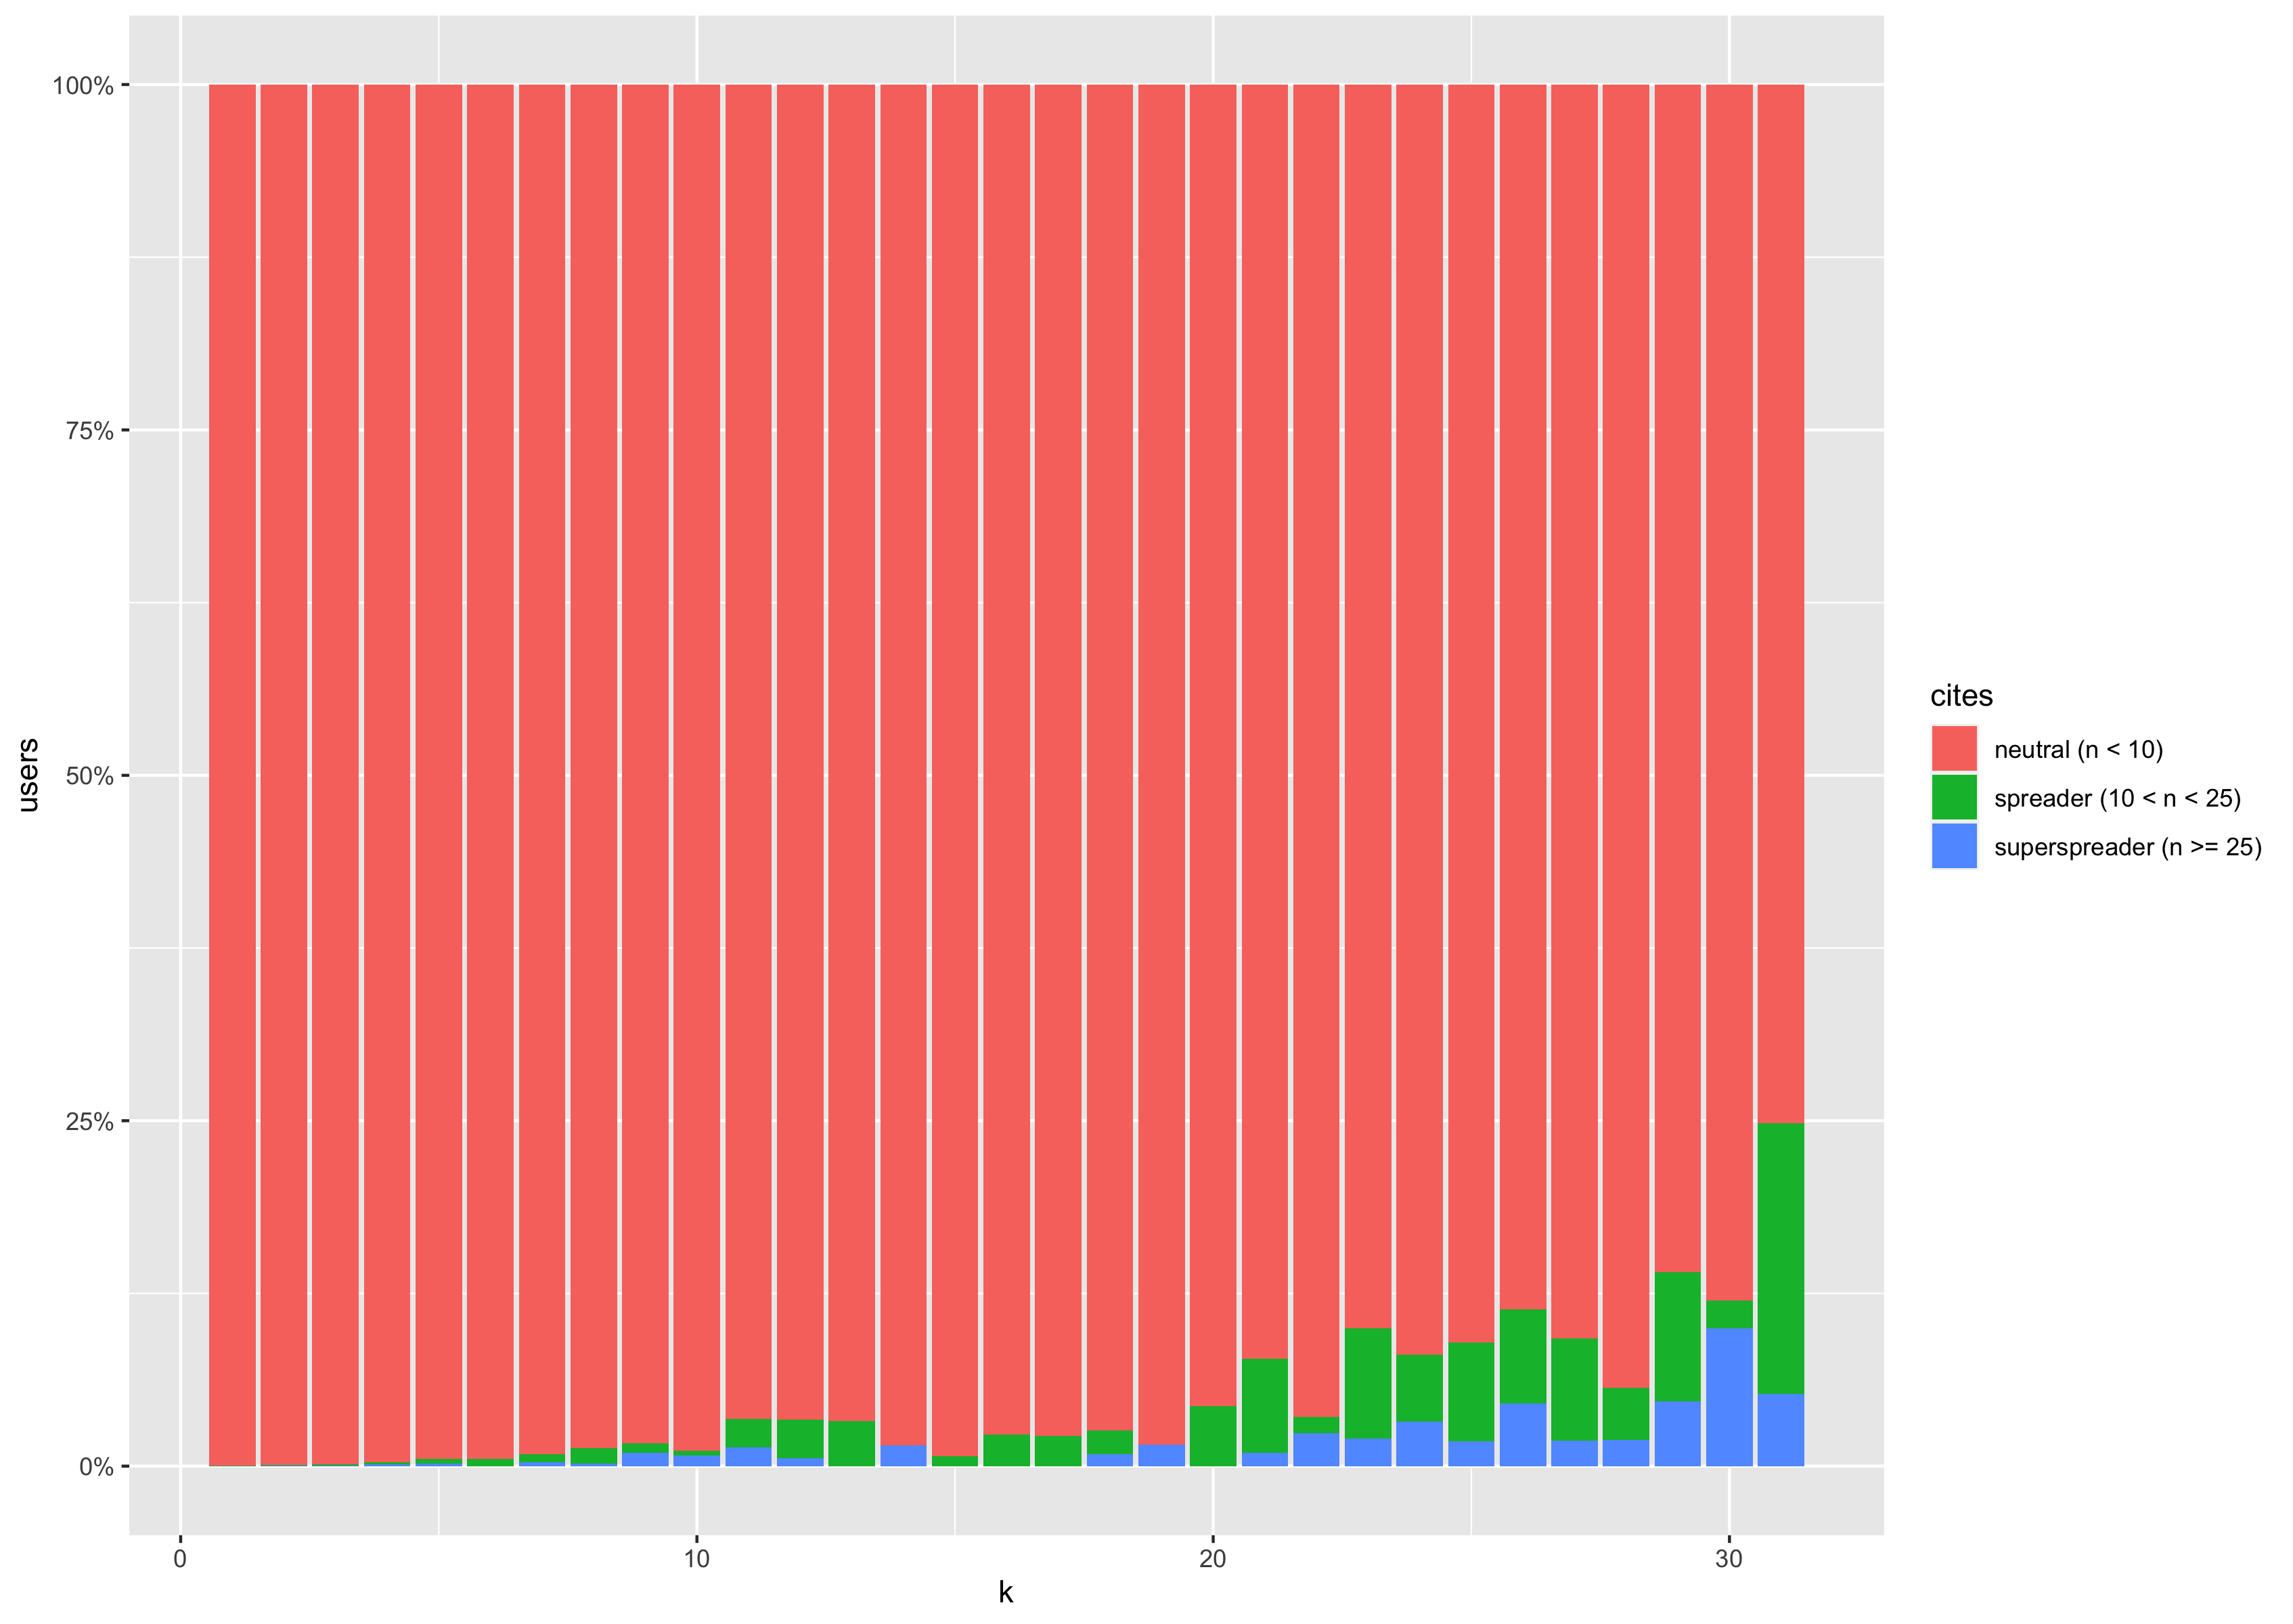
\includegraphics[width=\textwidth]{rus/kshells}
\caption{K-shells}
\label{fig:kshells}
\end{figure}

Figure \ref{fig:kshells} displays the k-core distribution.
The largest-connected component of the user network is composed of 59,009 users, 166 (0.28\%) are spreaders of Russian propaganda with at least 10 and less than 25 cites of domains in the combined Russian domain list, 66 (0.11\%) are superspreaders with at least 25 cites.
In total numbers (not depicted), neutral users have an extreme skew to the right with 53,808 (91.19\%) users located in the first 5 shells (on the periphery).
In contrast both the spreaders and superspreaders are more distributed in the higher shells; 168 (72.51\%) spreaders or superspreaders are found in shells 10 through 31, 132 (56.90\%) are found in shells 20 and higher, 76 (32.76\%) are found in the top shell, 26.66\% of all superusers.
Just as importantly, in the higher shells, rus users are a large percentage of all users, the top shell (31) is 24.87\% rus.
This indicates that Russian propaganda has reached positions of influence within the core of the network.

\begin{table}[!ht]
\footnotesize
\centering
\caption{Most ties in top k-shell}
\begin{tabular}{lrrllrl}
\toprule
 & ties & rus & top rus dom & top dom & cites & subreddit \\
user & & cites & & & & \\
\midrule
vigorous         &   856 &       1061 &      itar-tass.com &  itar-tass.com &    279 &          worldnews \\
holocauster-ride &   585 &         67 &              rt.com &  wikipedia.org &     91 &          worldnews \\
chewbacca81      &   574 &         18 &         rusvesna.su &  wikipedia.org &    145 &             russia \\
putupyourdukes   &   541 &          5 &   globalresearch.ca &  wikipedia.org &     50 &          worldnews \\
istinspring      &   483 &         34 &              rt.com &  wikipedia.org &    176 &             russia \\
Gibbit420        &   461 &         13 &              rt.com &  wikipedia.org &     75 &  UkrainianConflict \\
DisregardMyPants &   460 &         12 &              ria.ru &  wikipedia.org &     61 &  UkrainianConflict \\
spankaway        &   459 &          8 &              ria.ru &  wikipedia.org &     60 &  UkrainianConflict \\
4ringcircus      &   426 &          2 &              rt.com &  wikipedia.org &     13 &             russia \\
kornjacanasolji  &   415 &          6 &              mid.ru &  wikipedia.org &     43 &          worldnews \\
Glideer          &   408 &          9 &      newcoldwar.org &  wikipedia.org &     28 &  UkrainianConflict \\
Kuklachev        &   407 &          7 &              ria.ru &    youtube.com &     98 &  UkrainianConflict \\
kwonza           &   400 &          9 &               rg.ru &  wikipedia.org &     21 &          worldnews \\
ThePandaRider    &   378 &         10 &   globalresearch.ca &  wikipedia.org &     58 &  UkrainianConflict \\
WeAreBRICS       &   375 &         18 &              rt.com &  wikipedia.org &     35 &             russia \\
HighDagger       &   373 &         20 &         rusvesna.su &  wikipedia.org &    319 &          worldnews \\
JasonYamel       &   367 &          4 &            lenta.ru &  wikipedia.org &     69 &             europe \\
Infidius         &   356 &         14 &              rt.com &  wikipedia.org &     18 &          worldnews \\
turdovski        &   346 &         25 &  russia-insider.com &    youtube.com &    636 &             russia \\
kinmix           &   346 &          9 &              rt.com &  wikipedia.org &     57 &  UkrainianConflict \\
eugene7          &   345 &         13 &         lifenews.ru &    twitter.com &    104 &  UkrainianConflict \\
mkvgtired        &   340 &          6 &   globalresearch.ca &  wikipedia.org &     23 &             europe \\
9A4172           &   337 &          9 &              rt.com &    youtube.com &     21 &  UkrainianConflict \\
SpaceRaccoon     &   335 &         23 &      itar-tass.com &    youtube.com &    120 &             russia \\
orion4321        &   327 &          9 &  orientalreview.org &    youtube.com &    122 &  UkrainianConflict \\
Nilbop           &   326 &          6 &      itar-tass.com &  wikipedia.org &    116 &             europe \\
mrv3             &   323 &          8 &        infowars.com &  quickiwiki.com &     21 &          worldnews \\
LucifersCounsel  &   322 &         26 &              rt.com &  wikipedia.org &    182 &          worldnews \\
Vysotsky2        &   321 &         14 &              rt.com &    twitter.com &    112 &             russia \\
Rinnve           &   321 &         20 &           gazeta.ru &  wikipedia.org &     51 &          worldnews \\
\bottomrule
\end{tabular}

\label{tab:user_ties}
\end{table}

We further analyze the users of the top shell in Table \ref{tab:user_ties}.
The user with by far the most ties (856) with other users as well as citations of pro-Russian domains is the aptly-named u/vigorous.
This user is among 5 superspreaders in the top 30 with another 11 spreaders: rus users are 53.33\% of the 30 users with the most ties in the top shell.
15 prefer itar-tass.com, rt.com, or ria.ru out of our tagged Russian domains, but only u/vigorous cites them more than any other domain (279 times), and is one of 10 users whom post most often in the r/worldnews subreddit.
Unaware, non-partisan users are more likely to run into this biased content there than the other 3 subreddits favored by these top users.

Worth noting is the prevalence of Wikipedia.
21 of 30 users (70\%) cite it more than any other domain with 16 (53.33\%) of those citing it more than 50 times.
This presents a unique environment for the average user with no strong ties to or knowledge of the topic.
On the average thread some portion of it will contain users discussing the Ukrainian crisis with links to the at least nominally objective and accurate (and trusted) Wikipedia alongside disguised propaganda such as Oriental Review.
Oriental Review and users posting disinformation can either use complete falsehood or more-effectively (as the Wikipedia citations suggest) frame an event or fact in a way favorable to their position.

What dynamics are diving these user patterns?
Why is this relatively small set of users that post often salacious material from organizations out of the mainstream producing so much engagement?
It is probable that on a relatively niche (or non-salient) topic that this material does convince some of those that were uninformed.
However, it may be just as effective to divert the attention and resources of users with opposite positions by goading them on with controversy; by having the discussion there is the appearance of a contested concept, perhaps the main impression of the uninterested user.
King, Pan, and Roberts' research of the Chinese government's ``50c'' army shows ``strategic distraction'' itself has value \cite{king2017}.
Besides the noise it adds to the discussion, it is possible that trolling operations that are targeted internationally have a side-effect or goal of convincing domestic populations, too.
The r/russia subreddit, for example, provides an outlet to the West that may attract Russians at home and abroad; by virtue of being a foreign source it appears open but could be heavily manipulated.

\begin{table}[!ht]

\centering
\caption{Users by betweenness centrality}
\begin{tabular}{lrrrrll}
\toprule
 & bet & in & out & rus & dom & subreddit \\
user & cent z & deg z & deg z & cites & & \\
\midrule
holocauster-ride &       57.40 &     30.63 &      14.02 &         67 &   wikipedia.org &          worldnews \\
vigorous         &       52.42 &     26.16 &      45.72 &       1061 &   itar-tass.com &          worldnews \\
HighDagger       &       50.20 &     23.97 &       7.72 &         20 &   wikipedia.org &          worldnews \\
DisregardMyPants &       40.14 &     22.37 &       9.67 &         12 &   wikipedia.org &          worldnews \\
4ringcircus      &       34.59 &     21.42 &       7.49 &          2 &   wikipedia.org &             russia \\
chewbacca81      &       30.82 &     26.48 &      13.62 &         18 &   wikipedia.org &             russia \\
istinspring      &       30.63 &     26.88 &       9.60 &         34 &   wikipedia.org &             russia \\
putupyourdukes   &       30.47 &     24.51 &      13.60 &          5 &   wikipedia.org &          worldnews \\
Gibbit420        &       29.68 &     17.74 &      13.06 &         13 &   wikipedia.org &  UkrainianConflict \\
SpaceRaccoon     &       28.87 &     16.77 &      10.55 &         23 &     youtube.com &          worldnews \\
jaywalker32      &       28.73 &     14.79 &       5.76 &          8 &      reddit.com &          worldnews \\
vityok           &       27.20 &     12.80 &      12.20 &         23 &     youtube.com &             europe \\
varjag           &       27.14 &     12.56 &       4.04 &          2 &   wikipedia.org &  UkrainianConflict \\
mrv3             &       26.65 &     16.28 &       7.06 &          8 &   quickiwiki.com &          worldnews \\
angryteabag      &       25.63 &     12.65 &       5.51 &          2 &     youtube.com &          worldnews \\
kornjacanasolji  &       23.15 &     20.43 &       8.30 &          6 &   wikipedia.org &          worldnews \\
spankaway        &       22.67 &     25.87 &       7.95 &          8 &   wikipedia.org &  UkrainianConflict \\
RedWolfz0r       &       22.61 &     16.01 &       6.15 &          5 &   wikipedia.org &  UkrainianConflict \\
blurgtheamoeba   &       22.01 &      7.59 &       2.83 &          1 &   wikipedia.org &          worldnews \\
MonsieurAnon     &       20.73 &     18.20 &       5.96 &          0 &   wikipedia.org &          worldnews \\
zveroshka        &       19.15 &     11.50 &       4.41 &          2 &     youtube.com &          worldnews \\
kwonza           &       19.02 &     22.10 &       9.98 &          9 &   wikipedia.org &          worldnews \\
dubdubdubdot     &       18.92 &     14.09 &       3.32 &         31 &     youtube.com &          worldnews \\
BornInTheCCCP    &       18.75 &     13.17 &       4.93 &          2 &   wikipedia.org &  UkrainianConflict \\
Infidius         &       18.61 &     16.73 &      11.02 &         14 &   wikipedia.org &          worldnews \\
richmomz         &       18.30 &      9.08 &       7.26 &          5 &  theguardian.com &          worldnews \\
InternetFree     &       17.91 &      7.98 &       3.76 &          3 &   wikipedia.org &          worldnews \\
porlov           &       17.81 &     11.09 &       3.95 &          2 &   wikipedia.org &          worldnews \\
random\_racoon    &       17.74 &     16.08 &       6.91 &          7 &     youtube.com &          worldnews \\
iamadogforreal   &       17.72 &      6.24 &       5.44 &          0 &   wikipedia.org &          worldnews \\
\bottomrule
\end{tabular}

\label{tab:user_zs}
\end{table}

These particular users by generating lots of controversial content are likely to form the most connections in our undirected graph and therefore end up in the top cores of our k-core analysis.
It is useful to take a slightly different look at the graph via betweenness centrality.
Within a single connected component of a network each node has a shortest path (fewest connecting nodes) to every other node.
Nodes which end up on the shortest paths for the most node pairs score highly on betweenness centrality; these nodes serve as ``gatekeepers'' for the flow of information.
Degree affects this score in a similar manner to k-core analysis \cite[p. 201]{woolley2018}. 
Unlike the undirected graph used previously, when calculating this score we use a directed graph of users connected by replies.
In the case of reciprocal ties, the graph flows in the direction of the most replies.
Table \ref{tab:user_zs} displays the top 30 users by betweenness centrality.

Several of these values are expressed as z-score - the number of standard deviations from the mean; u/vigorous has a betweenness centrality score over 52.42 standard deviations from the mean, which means that they are located on the shortest path between other users many times above the average.
The average user in comparison will send and receive fewer responses and the responses they do receive will often be other less active users peripheral to the network.
They are one of the 16 users in this list (53.33\%) also counted among users with the most ties within the top k-shell in Table \ref{tab:user_ties}.
Every user has in and-out degree counts well above average but the ratio of in to out-degree varies.
5 are superspreaders of Russian propaganda with another 7 spreaders.
20 users cite Wikipedia more than any other site, 21 prefer r/worldnews, and the other subreddits (r/UkrainianConflict, r/russia, r/europe) are the same as those in the top k-shell.

\begin{table}[!ht]

\centering
\caption{Users by degree}
\begin{tabular}{lrrrrl}
\toprule
 & tot & in & out & rus & dom \\
user & deg z & deg & deg & cites & \\
\midrule
mrojek               &      60.32 &     117 &     5929 &          9 &  themoscowtimes.com \\
vigorous             &      43.59 &    1175 &     3202 &       1061 &      itar-tass.com \\
giggster             &      36.53 &     108 &     3565 &          6 &         reuters.com \\
Goobiesnax           &      29.64 &     224 &     2762 &          2 &      wikipedia.org \\
independentlythought &      28.79 &      14 &     2887 &          0 &         nytimes.com \\
TuEsiAs              &      26.29 &     122 &     2530 &          2 &        youtube.com \\
autowikibot          &      25.63 &    2446 &      140 &          7 &      wikipedia.org \\
holocauster-ride     &      23.41 &    1373 &      992 &         67 &      wikipedia.org \\
ionised              &      23.25 &      29 &     2320 &         16 &     theguardian.com \\
anutensil            &      23.05 &      12 &     2317 &         22 &         reddit.com \\
bobbybrown0503       &      22.27 &      12 &     2239 &          2 &     theguardian.com \\
chewbacca81          &      21.29 &    1189 &      964 &         18 &      wikipedia.org \\
live\_free            &      20.66 &     215 &     1875 &          0 &         reddit.com \\
putupyourdukes       &      20.40 &    1102 &      963 &          5 &      wikipedia.org \\
Buckfost             &      19.60 &      62 &     1923 &          2 &           imgur.com \\
Elizavetaisblue      &      19.48 &      58 &     1915 &          2 &        youtube.com \\
lobogato             &      18.96 &     444 &     1477 &          5 &  themoscowtimes.com \\
Den\_iz\_perf          &      18.93 &       8 &     1910 &          0 &  washingtonpost.com \\
istinspring          &      18.66 &    1207 &      684 &         34 &      wikipedia.org \\
Kuklachev            &      18.65 &     710 &     1180 &          7 &        youtube.com \\
uptodatepronto       &      18.41 &      45 &     1821 &         14 &        twitter.com \\
AkitaBijin           &      18.37 &      72 &     1790 &          2 &           rferl.org \\
jlew24asu            &      18.32 &      30 &     1827 &          0 &         reuters.com \\
eu\_ua                &      18.08 &     197 &     1636 &          1 &         google.com \\
i\_love\_fsa           &      17.87 &      16 &     1796 &         20 &    dailystar.com.lb \\
spankaway            &      17.06 &    1162 &      569 &          8 &      wikipedia.org \\
Gibbit420            &      17.02 &     802 &      925 &         13 &      wikipedia.org \\
kwonza               &      16.80 &     995 &      710 &          9 &      wikipedia.org \\
DisregardMyPants     &      16.71 &    1007 &      689 &         12 &      wikipedia.org \\
Madbreakfast         &      16.63 &     152 &     1537 &          1 &        twitter.com \\
\bottomrule
\end{tabular}

\label{tab:user_deg}
\end{table}

Finally, Table \ref{tab:user_deg} displays a slightly different view of the same data, the top 30 users by total degree.
The same subreddits are present, but the set of domains and users is more diverse, only 10 have more than 10 cites of rus domains.
The majority of users in this list have high out-degree especially compared to in-degree.
However, several of the users, especially the superspreaders, have high, or inflated, in-degrees. 
The superspreaders u/holocauster-ride (1,373/992) and u/istinspring (1,207/684) have significantly more incoming connections than outgoing; u/vigorous, despite having 3,202 outgoing connections compared to the 5,929 of the neutral user u/mrojek, has 1,058 more incoming connections.

Overall, no matter which network measure we use, propaganda appears to exist at all levels in slightly different forms.
Similar users, domains, an emphasis on Wikipedia, and subreddits are apparent. Some users are much more effective than others at getting reactions (those in the top k-shells), but a number of users are very active without a lot of incoming responses.
Is this behavior naturally occurring or intentional?
Does outrageous material happen to cause reactions or is it selected and posted because of that virality?
Is r/worldnews prominent because it is a featured subreddit or is it targeted because of that?
To know whether these questions matter, we need to better understand the nature of the content being posted through textual analysis.
We have identified pro-Russian users and seen that they are located in the core of the network, the next step is to find out what topics they are discussing and whether this discussion is noticeably different form neutral users.

\subsection{Textual Analysis}

It was the growth of the tech industry and social media after 2000 which produced the dynamics for computational propaganda and generated textual data at a scale never before seen.
This in turn produced the need for tools to process these massive amounts of (big) data and the resources to produce these tools in the form of the machine learning (artificial intelligence) revolution.
Specifically, more accurate models of representing language were developed that better understood context and meaning.
In 2013, a team led by Tomas Mikolov at Google published Word2vec \cite{mikolov2013}.
Technically, Word2vec uses a shallow 2-layer neural network to produce word embeddings; because there is an abundance of material that already explains similar machine learning methods, we refer to them and view Word2vec as a black box, as a machine that we feed data into and from which we get results.

Word2vec is trained with a large amount of textual data.
With each document fed in for training, Word2vec updates its model and understanding of how individual words relate to each other by representing each individual word as a vector (list, array, sequence) with a decimal value for any number of dimensions, these word vectors are ``embedded'', exist in a ``vector space''.
Usually there are hundreds of dimensions, one for each abstract attribute of the word, by this we are able to efficiently and accurately use mathematical operations on the vectors and therefore the word.
For example, \emph{kitten = dog - puppy + cat}.
Upon training a Word2vec model, it can be queried to get a ranked list of most or least-similar words.

\begin{table}[!ht]
\centering
\caption{Word vectors}
\begin{tabular}{rr}
\toprule
   friend &     enemy \\
\midrule
 0.070801 &  0.306641 \\
-0.213867 &  0.034180 \\
 0.153320 &  0.019531 \\
 0.094238 &  0.192383 \\
-0.034424 & -0.382812 \\
 0.433594 &  0.287109 \\
-0.165039 & -0.157227 \\
-0.057861 &  0.051270 \\
 0.175781 &  0.208984 \\
-0.082031 &  0.267578 \\
\bottomrule
\end{tabular}

\label{tab:friend1}
\end{table}

\begin{table}[!ht]
\centering
\caption{Most-similar terms}
\begin{tabular}{ll}
\toprule
       friend &                     enemy \\
\midrule
          pal &                   enemies \\
      friends &                 adversary \\
        buddy &               adversaries \\
  dear\_friend &                  hostiles \\
 acquaintance &         old\_Mariam\_Sajadi \\
       cousin &      inevitably\_Schulberg \\
   girlfriend &        heartless\_ruthless \\
    colleague &     must\_outthink\_outwork \\
        uncle &  Islamofascist\_terrorists \\
     roommate &                aggressors \\
\bottomrule
\end{tabular}

\label{tab:friend}
\end{table}

To show this in a more concrete and political context, we use a freely-available model from Google that has been trained on about 100 billion words from a news dataset.
For our input (not training) data we use the line from Lincoln's first inaugural address, ``We are not enemies, but friends. We must not be enemies''.
Common text cleaning techniques will often filter out most of these words; Table \ref{tab:friend1} displays 10 dimensions of the vector representations and Table \ref{tab:friend} the 10 most-similar words for ``friend'' and ``enemy''.

These results mostly present associations that humans would naturally make, they also tell a lot about the training data used.
There are singular and plural forms of the same word, varied casing, and underscores; whether this level of text cleaning and filtering is acceptable comes down to familiarity with the data as well as intended goals.
Cleaning is a boring but necessary process, because of this some introductions and guides understate how very trial and error-intensive it can be.
Feeding ``bad'' (unrepresentative, inaccurate) data into a model will usually produce ``bad'' results.
In that case, that worked for Google for an example dataset.
For our own needs, we will train our own models based on populations (groups) of users in the Reddit data.

\begin{table}[!ht]
\centering
\caption{User groups}
\begin{tabular}{lrrrrrr}
\toprule
{} & users & doms & comment & comment & submission &  submission \\
group         &  &  & matches & relatives & matches & relatives \\
\midrule
neutral       &  193647 &  346457 &           381264 &             776965 &               39312 &                 52842 \\
superspreader &      75 &   43239 &            13201 &              16223 &               13280 &                  3118 \\
top           &  117383 &  191927 &           246513 &             463195 &               18875 &                 48024 \\
totals        &  193910 &  458107 &           459054 &            1033697 &               87008 &                 72688 \\
\bottomrule
\end{tabular}

\label{tab:group1}
\end{table}

Table \ref{tab:group1} displays basic stats about these groups: the number of users within, how many domains they post, and the quantity of matches and relatives for both submissions and comments.
We reuse the existing neutral and superspreader user groups based on the number of pro-Russian citations.
The groups offer competing ideologies, we want to know to what extent the average discussion on relevant topics corresponds to or is apparently influenced by each group.
Short of a controlled testing environment, it is difficult to determine what the average user will read, pay attention to, or remember for a given Reddit submission with comments.
In order to approximate interest, we create a new ``top'' users group consisting of all matches and related items that have at least a single reply to them.
Items that have no responses have not motivated anyone to take action, positive or negative, by excluding them we get the topics and content that are drawing interest.

The text portion of each item (title and selftext for submissions, body for comments) is processed by spaCy and each word is converted to its lemma, the base word.
Stopwords (the, and, it, etc) are removed and separate Word2vec models are trained for each group using the processed data and the Gensim Python library; these trained models can then be used to compare associations made with various terms (words) across these different sets of users.

We use t-SNE (t-distributed stochastic neighbor embedding) to reduce the word vector's 300 dimensions down to a two-dimensional projection that is easy to visualize.
Ideally, words more closely related to each other are closer together, but with each graph we are looking at a limited 2D slice \cite{van2008}.
We separately use k-means on the vectors to group the terms into k clusters of terms that are used commonly with each other. 
Ultimately, what Word2vec captures and we are able to observe is which words are found in close physical proximity in the text, this is their ``similarity''. \footnote{The Gensim Python library is once again used here, but both t-SNE and k-means are well-understood algorithms implemented in a number of languages.
The basis of progress in many fields, but especially programming, is that the user does not have to know how a program (or its parts) work, in the same way you do not have to know how a car engine works to drive a car.
The user does need to know their goals (dimensionality-reduction), the expected inputs (vectors of many dimensions), outputs (vectors of two-dimensions, points), consequences (reducing dimensionality means losing information), and common mistakes (k-means similarly works on many dimensions, so using 300 is better than 2).
These are small machines that can be understood separately, plugged together, and need little programming knowledge.}

Considering that t-SNE was published in 2008 and Word2vec in 2013, the ability to visualize text and its associated meaning in this manner is relatively new. 
It is tempting, especially with the direct mapping of words to numeric values to treat it as a kind of scientific numerology or for it to be a Rorschach test. We cannot make absolute statements about meaning as we have intentionally removed dimensions, information to build the plot.
However, there is apparent face-validity and using domain knowledge we can identify patterns and make observations.
For clarity, terms in the context of Word2vec are \emph{italicized} going forward.

\begin{figure}[!ht]
\centering
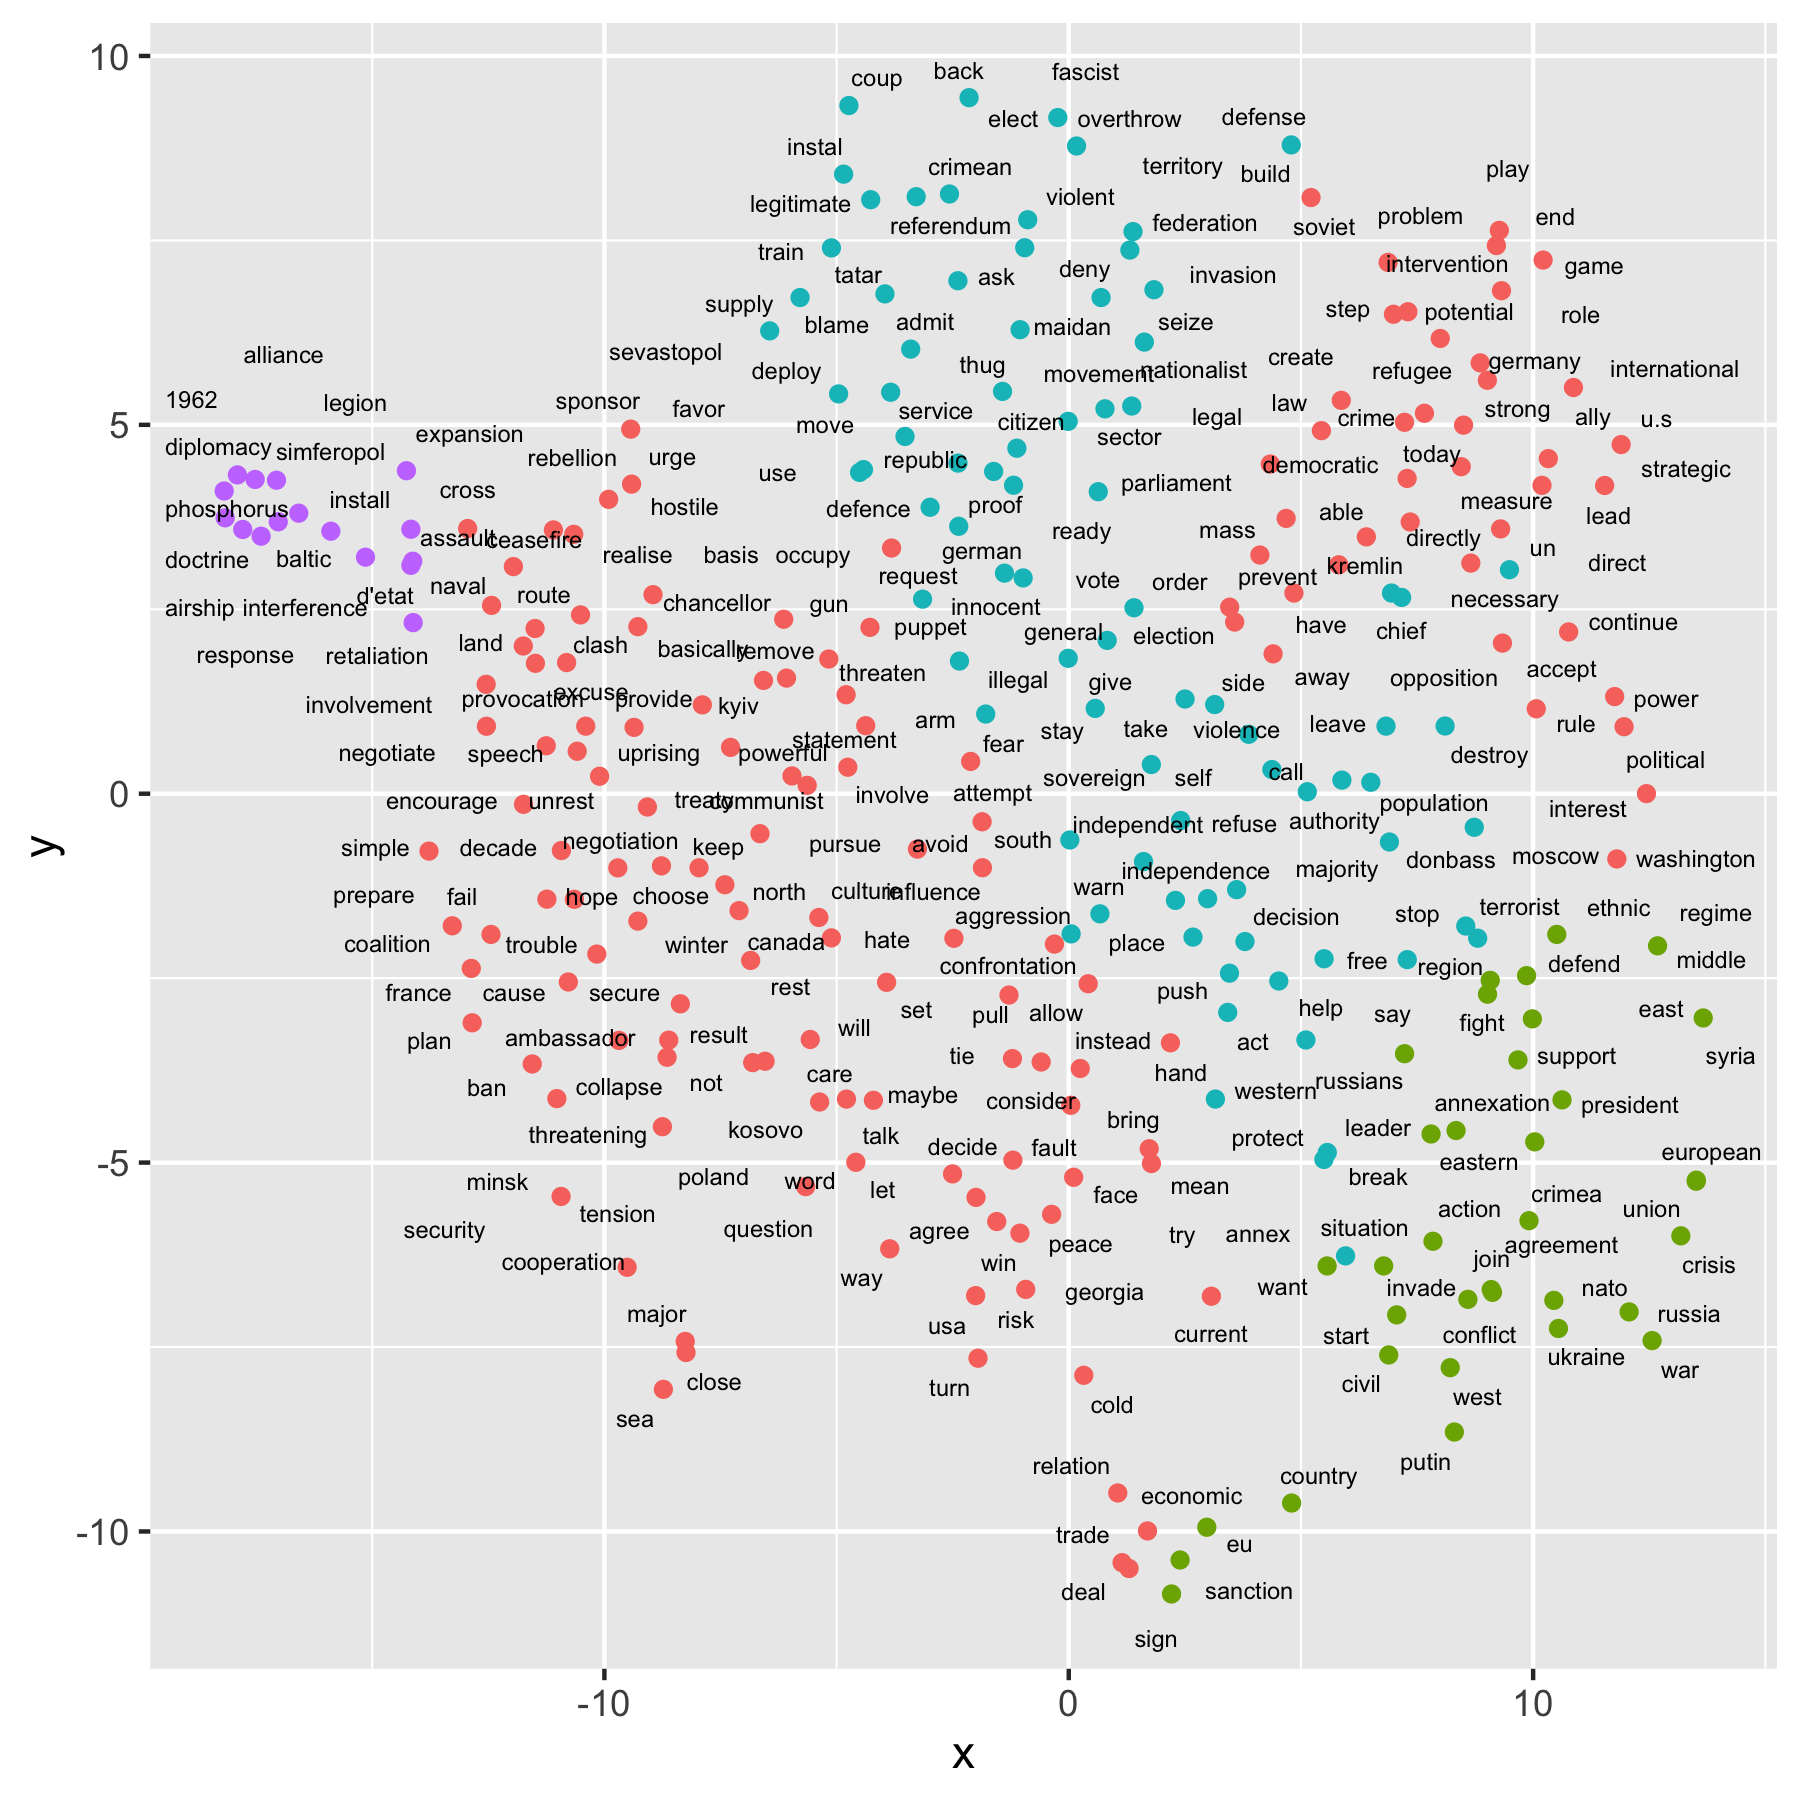
\includegraphics[width=\textwidth]{rus/superspreader_putin}
\caption{Most-similar to ``putin'' (superspreaders)}
\label{fig:superspreader_putin}
\end{figure}

The following figures display the most-similar words for ``putin'' for selected terms across two groups.
In Figure \ref{fig:superspreader_putin}, there are 287 terms; because Word2vec discovers relationships, terms cluster both by ``personness'' and other factors, we remove 13 names of individuals to avoid this.
There is no optimal k for the number of clusters, but the clustering remains similar using various options and the superspreader group presents similar plots using different terms: \emph{putin, crimea, ukraine}.
The term \emph{putin} is located near 8.3, -8.65, its surrounding cluster contains the entities he is in direct competition with: \emph{west, nato, ukraine, european, union, eu}, using various means: \emph{conflict, war, sanction, agreement, invade, defend, fight, support, action, russia}, over objects of contention: \emph{crimea, russians, middle, east, eastern, region, syria}.

The cluster at -15, 2 includes pointed arguments: \emph{1962}, the year of the Cuban Missile Crisis, and claims of \emph{phosphorous}.
Split across -10, -5, and 10, 5 is an international cluster of secondary actors and issues: \emph{france, germany, kremlin, u.s, ally, ambassador, chancellor, poland, kosovo, georgia} and less concrete actions and notions: \emph{speech, provocation, negotiate, encourage, prepare, strategic, prevent, power}.
Finally, the cluster located at 0, 10 is a series of terms that match Russian talking points, painting the new government of 2014 as nazis denying popular will: \emph{coup, fascist, maidan, puppet, nationalist, movement, thug, overthrow, sector, illegal, legitimate, instal, sovereign, independent, referendum, majority, population, donbass}.

\begin{figure}[!ht]
\centering
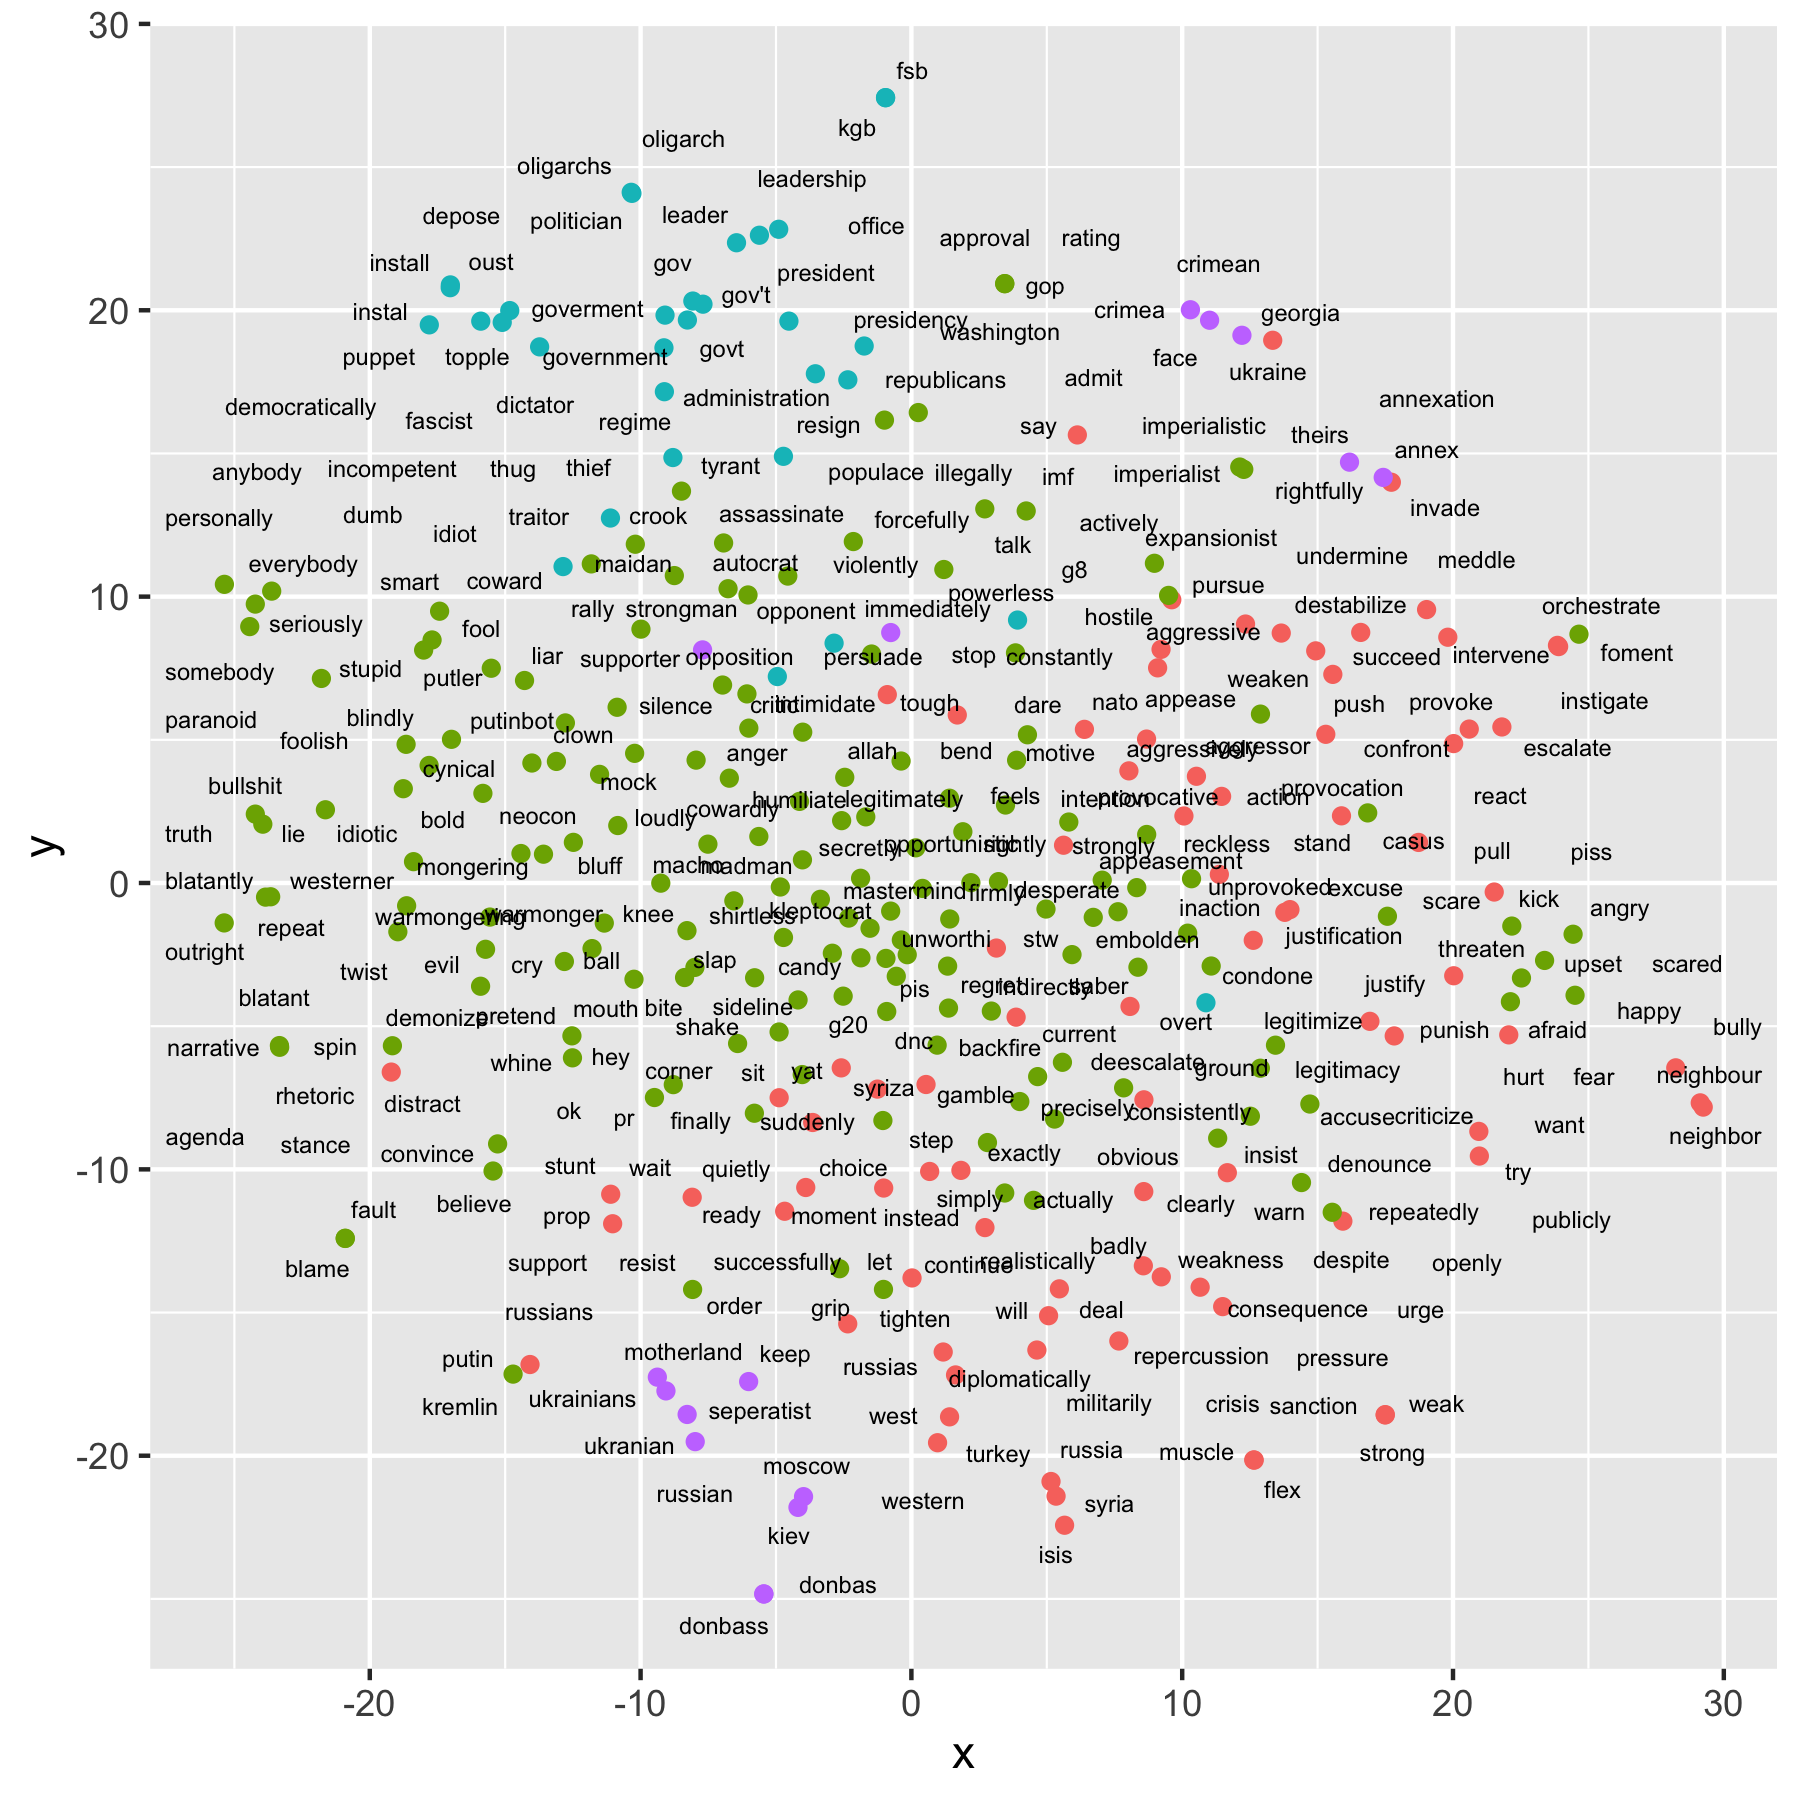
\includegraphics[width=\textwidth]{rus/neutral_putin}
\caption{Most-similar to ``putin'' (neutral users)}
\label{fig:neutral_putin}
\end{figure}

In comparison, the neutral users plot of Figure \ref{fig:neutral_putin} presents similar clusters with a different emphasis.
This group is dominated by individuals; 316 terms are displayed with 84 excluded.
We locate \emph{putin} near -14, -16; nearby is a cluster of relevant parties: \emph{ukrainian(s), moscow, kiev, donbas(s), crimea(n), separatist}.
The international cluster (10, -20) of actions remains, though it tends to be more negative: \emph{pressure, bully, neighbor, hurt, punish, weakness, repercussion, crisis, unprovoked, aggressive}.
Similarly, the cluster at -10, 2 focuses on a puppet government, though it is not obvious to which government it is referring: \emph{puppet, government, topple, fascist, dictator, depose, install, oust, thug, oligarch(s), kgb, fsb}.
The most obvious difference is found in the central \emph{putin} cluster, where the majority of the terms are very negative: \emph{stupid, idiotic, foolish, paranoid, bullshit, demonize, evil, madman, liar, fool, putler, clown, coward(ly), desperate, warmongering}.
Clearly, these different groups display strong differences in narrative and opinion; to determine whether either group is representative of discussion we look at different terms in the top users group.

\begin{figure}[!ht]
\centering
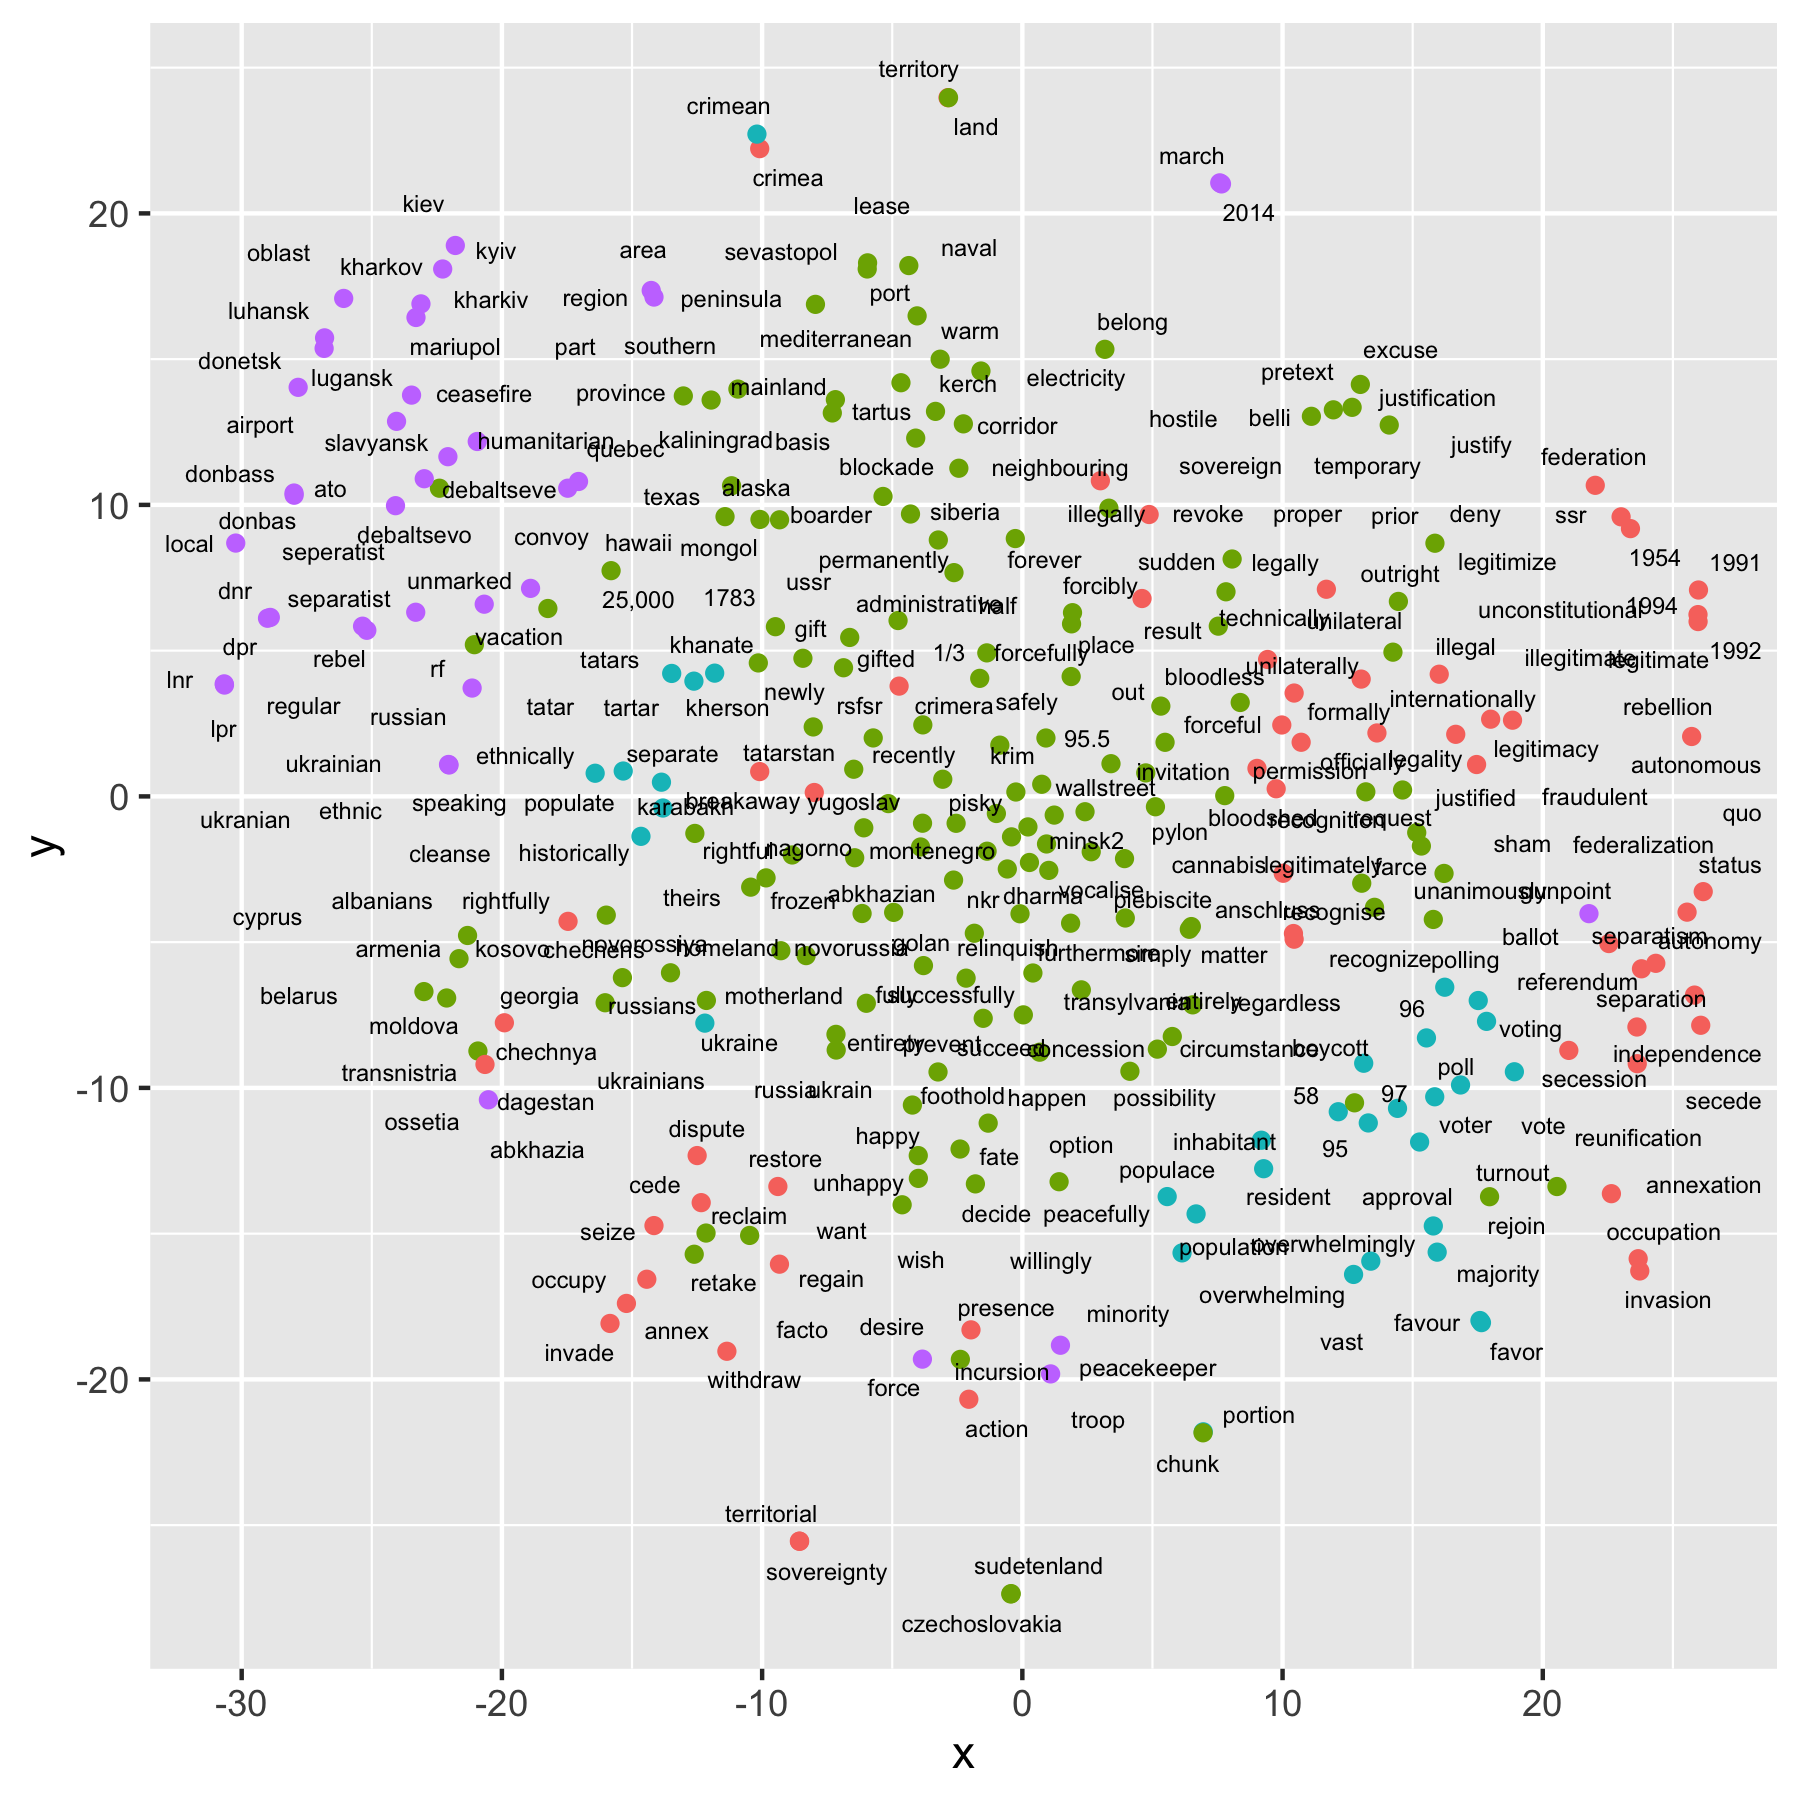
\includegraphics[width=\textwidth]{rus/top_crimea}
\caption{Most-similar to ``crimea'' (top users)}
\label{fig:top_crimea}
\end{figure}

\begin{figure}[!ht]
\centering
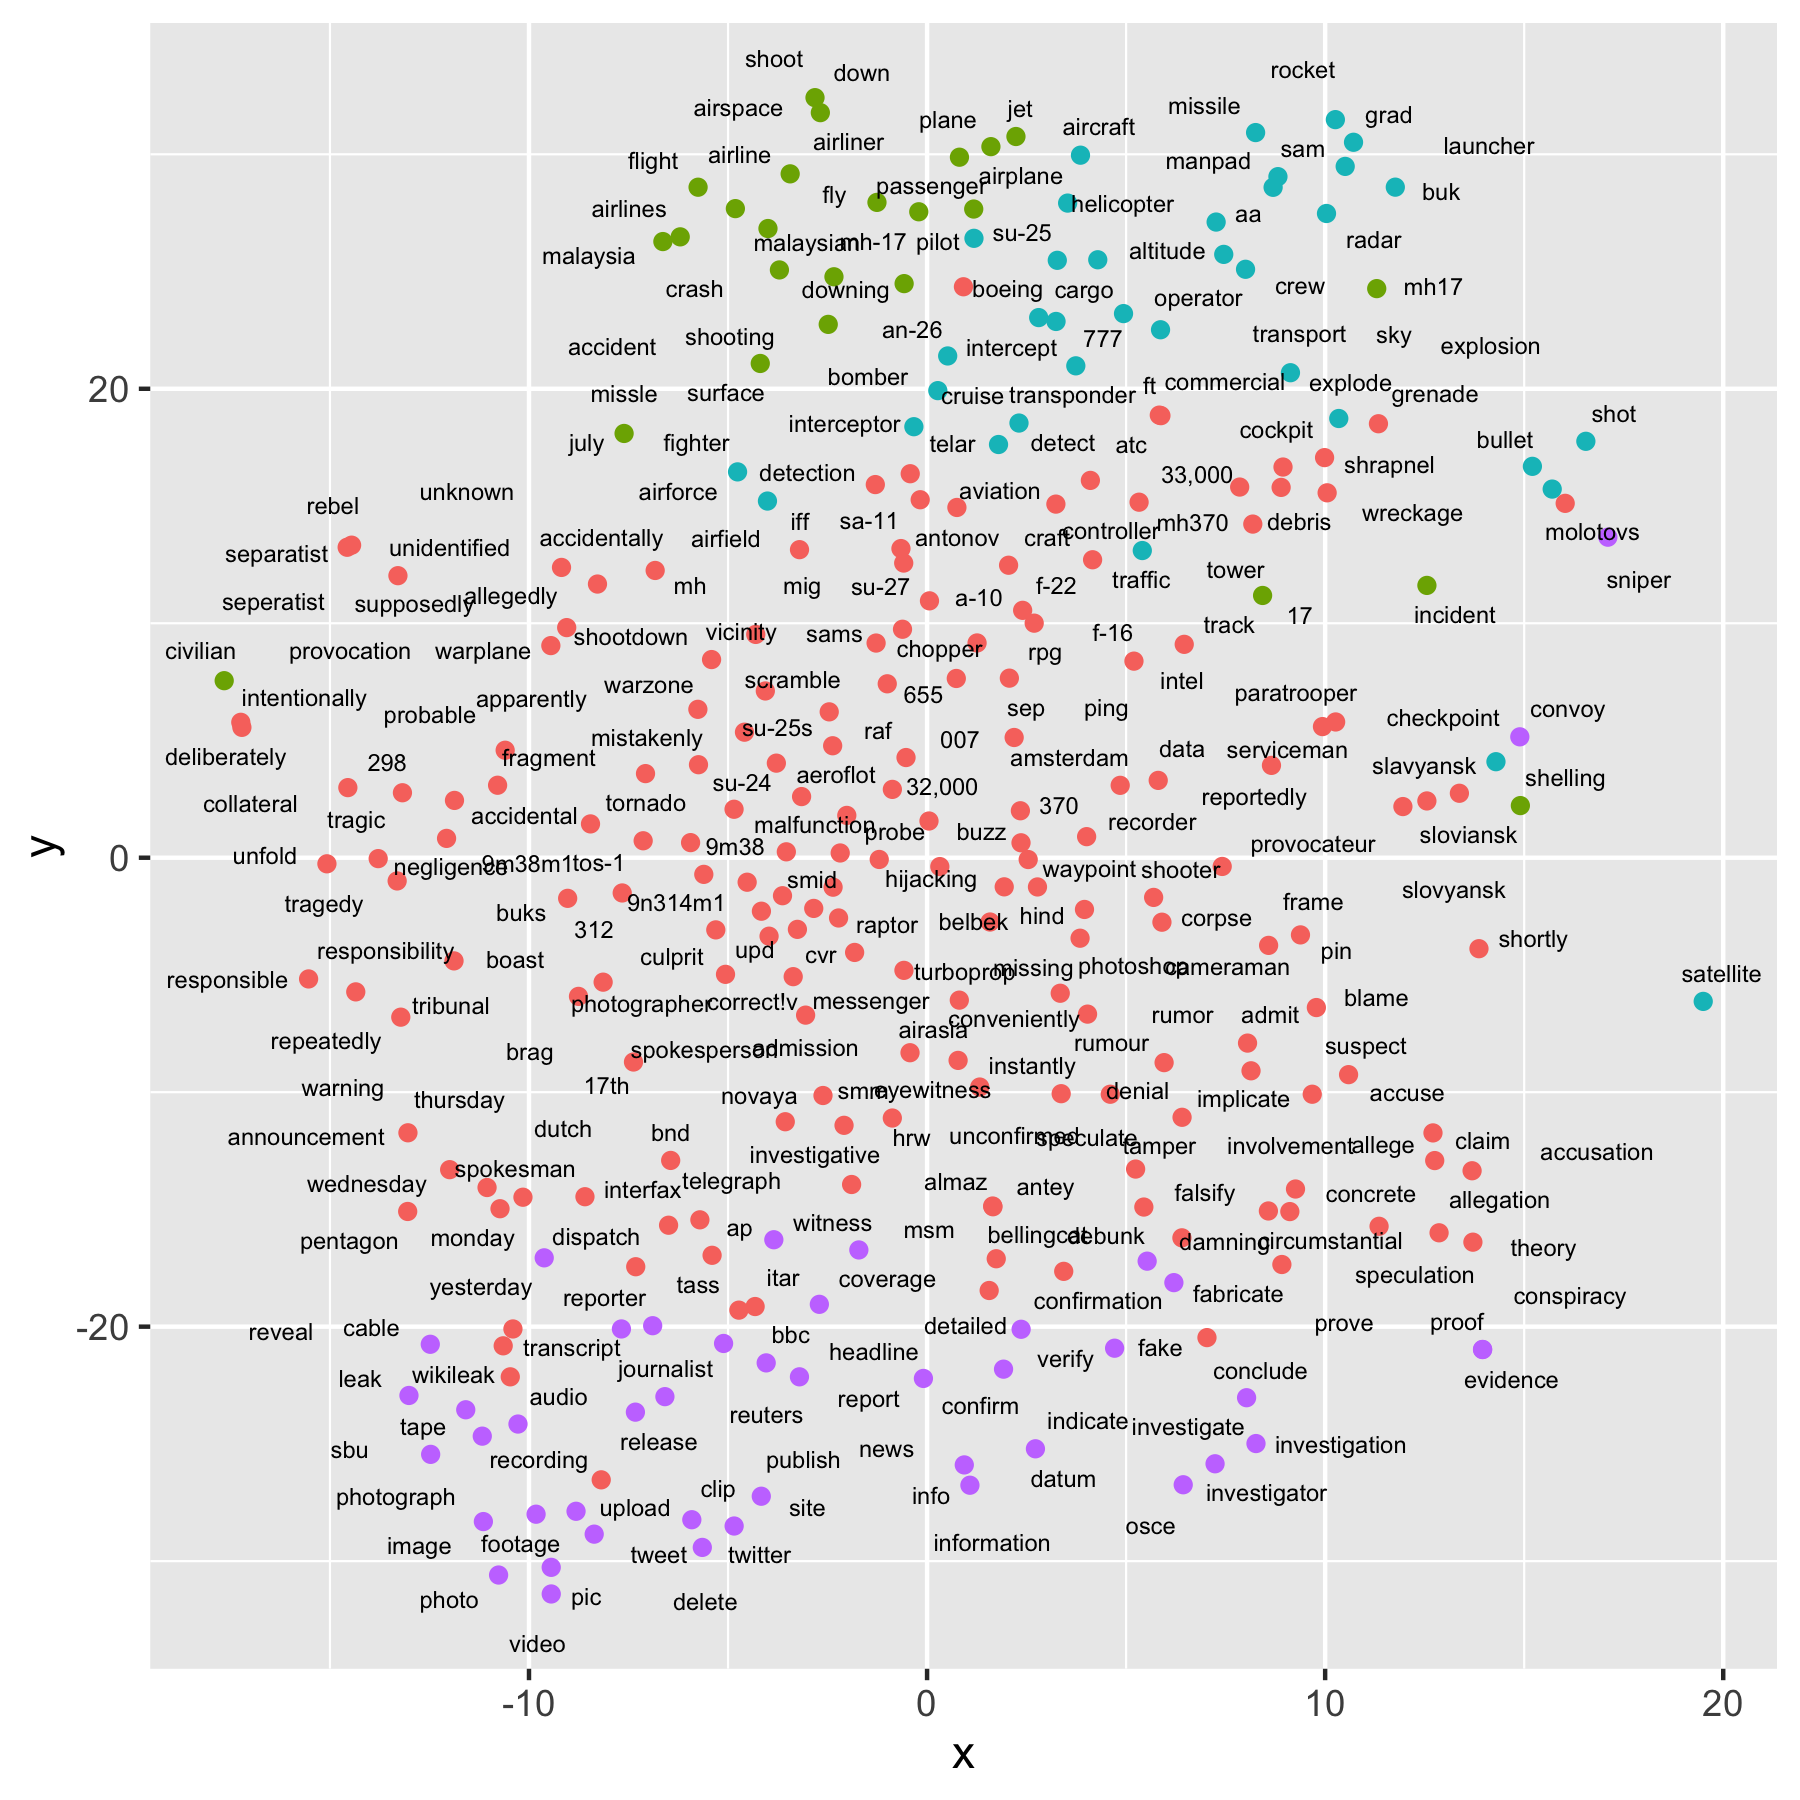
\includegraphics[width=\textwidth]{rus/top_mh17}
\caption{Most-similar to ``mh17'' (top users)}
\label{fig:top_mh17}
\end{figure}

Figures \ref{fig:top_crimea} and \ref{fig:top_mh17} show most-similar terms for the top users group.
The first graph displays the 294 most-similar terms for ``crimea'' with 6 terms excluded.
The cluster at -20, 10 contains the reality on the ground with Russian-backed republics established by separatists in the Donbass region: \emph{separatist, ceasefire, donbas(s), donetsk, luhansk, oblast, march, 2014}.
The term \emph{crimea} is found nearby at -10, 20, but most of its cluster is located at 25, -10 with a discussion of the legalities involved: \emph{secession, federalization, legitimacy, fraudulent, autonomous, unconstitutional, reunification}, relevant years: \emph{1991, 1992, 1994, referendum}, and \emph{1954, ssr}, the year Ukraine was attached to the Ukrainian SSR.
The nearby cluster at 10, -15 continues the topic of voting: \emph{population, populace, willingly, peacefully, overwhelming(ly), vote(r), poll(ing), favor}, reflecting the Russian populace of the region, and at -15, 0, remembering that those demographics were recent: \emph{historically, populate, ethnic, cleanse, tatar(s), khanate}.
The last cluster at 0, 0 has a similar historic tilt: \emph{1783, novorussia, warm, port, sevastapol}, and transparent attempts to connect the annexation of Crimea to other historic annexations and existing independence movements: \emph{hawaii, texas, alaska, kosovo, quebec}, yet also contains more recent, more negative analogs: \emph{sudetenland, anchluss, czechoslovakia}.

In Figure \ref{fig:top_mh17}, there are 286 terms with 14 excluded; ``mh17'' is found near 10, 25, its cluster is at -5, 25 with a straightforward account: \emph{malaysia, airlines, accident, shooting, downing, crash}.
The cluster at 5, 25 gives more details: \emph{buk, missile, sam}, the Buk was the Russian-supplied missile system used by separatists (probably commanded by Igor Girkin) to destroy the plane.
The cluster found at 0, -10 is concerned with the investigation: \emph{image, photograph, footage, clip, site, report, bbc, itar, reuters, tweet, twitter, journalist, transcript, confirm, evidence}, as is the main cluster located at 0, 0, with the \emph{dutch} investigative team that confirmed the separatist shoot down as well as \emph{bellingcat}, an investigative team dedicated to debunking misinformation.
Distributed around the cluster is the \emph{conspiracy theory} given by the supposed \emph{traffic controller} at an \emph{airfield tower} in Ukraine that saw an Ukrainian \emph{su-24} in the \emph{vicinity} of the shoot down, an account promoted by Russian media.

For the Putin plots, both superspreaders and neutral users contain abstract terms related to Putin himself as well as a variety of details about the Ukrainian and Crimean conflict.
The biggest and expected difference is in the many negative references found in the neutrals but missing from the superspreaders

In comparison, the plots of the top users (or users that are getting responses), while including relevant details also contain a large number of terms related to Russian talking points.
For example, the many dates and references to annexation in the Crimea plot and stories distributed by the Russian MoD and media regarding MH17.
This mixed group of active discussion we might expect to be less colored than the actual Russian superspreaders is instead the most-framed.
It makes sense that the act of communication and debate between two groups brings out more information, this suggests that the best way to combat disinformation is not to target ideological groups but rather to ensure valid, factual information is there to counter the misleading when discussions happen.

\section{Discussion}

In this chapter we discussed how a combination of dynamics - the fall of the Soviet Union, rise of the Putin regime, and growth of the tech industry across the world led to an embrace of computational propaganda by the Russian government.
Computational propaganda was combined with asymmetric warfare, covert operations such as poisonings, and hacking and misinformation campaigns to produce the so-called Gerasimov doctrine.
This was first tested at scale in Ukraine from 2013 to 2014 leading up the the Crimea's annexation by Russia.
We use the existing academic literature about this crisis and general tactics of Russian ``trolls'' across social media including Facebook and Twitter in order to guide our analysis of the crisis using the Reddit dataset.

We clean the dataset, process it using spaCy, then use a basic filtering scheme checking for the presence of terms like ``putin'' and ``crimea'' to find matched and related items.
The dataset is further filtered using a set of rules regarding subreddits in order to exclude irrelevant data.
The resulting data shows spikes in activity corresponding closely with the main events of the crisis - the abdication of Yakunovych and annexation of Crimea, the downing of MH17, and the Minsk II ceasefire.

Next, we use a simple categorization scheme using web domain addresses in order to put content and users into neutral and pro-Russian groupings, filtering out apparent bots.
This involves a combined list of ``core'' Russian (and Chinese/Iranian) state-owned domains and outlets and an ``extended'' list of domains across the political spectrum known for parroting Kremlin talking points or conspiracy theories, some more covertly or intentionally than others.
Users with at least 10 cites of a domain in this list across the 3 years are known as ``spreaders'' of pro-Russian content and those with more than 25 are ``superspreaders''.
We find that while discussing this topic users generally cited a variety of US, British, Ukrainian, other international, and Russian outlets with Russian state media being prominent.
Pro-Russian users seem to favor niche, low-credibility sources.
Users cited Wikipedia more than any other domain with many references to analogous historical events.

In order to observe patterns in activity as well as the possible reach of the pro-Russian users, we use several methods from graph theory and network analysis.
The first, k-core analysis, confirms the presence of pro-Russian users in the highest shells of users with the most connections to other users in the network, with spreaders and superspreaders found heavily clustered in the top k-core.
These same superspreaders similarly dominate top measures of betweenness centrality and total degree (number of connections) and show an apparent preference for a handful of subreddits and for citing Wikipedia.
These various measures suggest that pro-Russian propaganda has achieved positions of influence in the network, allowing for easy dissemination.

Finally, we train our own Word2vec models.
By training separate models for different groups of users we are able to compare word associations of a given term across them.
This is achieved by dimensionality reduction in order to plot terms on a two-dimensional graph with points clustered via k-means.
In the case of the term \emph{putin}, neutral users present a cluster of negative terms which is absent for the superspreaders.

These different groups show a different focus, but to capture which narratives dominate the average discussion, we create a final group of ``top users'', containing only items that have at least a single reply.
Both \emph{crimea} and \emph{mh17} include clusters with straightforward accounts as well as a relatively nuanced description of various connected issues.
However, these accurate accounts are distributed among pointed historic and legal arguments, as well as conspiracy theories promoted by the Russian state.

We note the apparent effectiveness of the framing of these issues - the exact same event or notion can be used to support wildly different positions.
Whether framing in this data is the result of an intentional campaign or just obsessive users is difficult to say, though users including u/vigorous post an unusually high number of items.
We note the apparent presence of power laws in the dataset.
Zipf's law, commonly applied to textual data, says that in a large enough body of text the term used most frequently will be used twice as often as the second most used term, three times as often as the third, and so on; or, the frequency of a term is inversely proportional to its rank.
Zipf has been more generally applied to other human interactions, this clustering activity seems to be a feature of human behavior.
The practical result of most discussions being limited to a few subreddits, most citations involving the same domains or articles, and a relatively limited number of topics means that it would take very few users to control and direct discussion, to have outsized influence.
Compounding this is the difficulty of knowing what varied demographics with their own beliefs, biases, and knowledge bases will notice and prefer when presented the average Reddit thread, news article, or equivalents of clusters of terms.

The end result of this chapter has been the development of a general framework for filtering and categorizing a large textual dataset.
For any group of users across any topic we can distill the combined text into a visualization of several hundred words, graphs of talking points.
Next, we apply this framework to the 2016 US presidential election.
